%%%%%%%%%%%%%%%%%%%%%%%%%%%%%%%%%%%%%%%%
%%%%% NATURE CLIMATE CHANGE FORMAT %%%%%
%%%%%%%%%%%%%%%%%%%%%%%%%%%%%%%%%%%%%%%%
%% Comment "% WPcomment" lines, uncomment "% NCCcomment" lines as well as the lines below, replace all citet/citep by cite

% \documentclass{nature}
% \usepackage{amsmath}
% \usepackage{amssymb}
% \usepackage{eurosym}
% % The following allows keeping figures within the text (otherwise nature.cls would ignore them)
% \usepackage{graphicx}
% \makeatletter
% \let\saved@includegraphics\includegraphics
% \AtBeginDocument{\let\includegraphics\saved@includegraphics}
% \renewenvironment*{figure}{\@float{figure}}{\end@float}
% \makeatother

% Nature guidelines (not NCC!)
% Sections can only be used in Articles.  Contributions should be organized in the sequence: title, text, methods, references, Supplementary Information line (if any), acknowledgements, interest declaration, corresponding author line, tables, figure legends.

% No subsubsection nor paragraph

% Spelling must be British English (Oxford English Dictionary)

%Each figure legend should begin with a brief title for the whole figure and continue with a short description of each panel and the symbols used. For contributions with methods sections, legends should not contain any details of methods, or exceed 100 words (fewer than 500 words in total for the whole paper). In contributions without methods sections, legends should be fewer than 300 words (800 words or fewer in total for the whole paper).

% Articles are restricted to 50 references,

% In addition, a cover letter needs to be written with the
% following:
% \begin{enumerate}
%  \item A 100 word or less summary indicating on scientific grounds
% why the paper should be considered for a wide-ranging journal like
% \textsl{Nature} instead of a more narrowly focussed journal.
%  \item A 100 word or less summary aimed at a non-scientific audience,
% written at the level of a national newspaper.  It may be used for
% \textsl{Nature}'s press release or other general publicity.
%  \item The cover letter should state clearly what is included as the
% submission, including number of figures, supporting manuscripts
% and any Supplementary Information (specifying number of items and
% format).
%  \item The cover letter should also state the number of
% words of text in the paper; the number of figures and parts of
% figures (for example, 4 figures, comprising 16 separate panels in
% total); a rough estimate of the desired final size of figures in
% terms of number of pages; and a full current postal address,
% telephone and fax numbers, and current e-mail address.
% \end{enumerate}

% See \textsl{Nature}'s website
% (\texttt{http://www.nature.com/nature/submit/gta/index.html}) for
% complete submission guidelines.

%%%%%%%%%%%%%%%%%%%%%%%%%%%%%%%%
%%%%% WORKING PAPER FORMAT %%%%%
%%%%%%%%%%%%%%%%%%%%%%%%%%%%%%%%
%% Comment "% NCCcomment" lines, uncomment "% WPcomment" lines as well as the lines below
\documentclass[12pt,english]{article}
\usepackage[utf8]{inputenc}
\usepackage{tgpagella} % Palatino text only
\usepackage{mathpazo}  % Palatino math & text
\usepackage[left=1.5in,right=1.5in,top=1.5in,bottom=1.5in]{geometry}
% \linespread{1.5}
\usepackage[super,comma,sort]{natbib} % WPcomment
% \usepackage[round,sort&compress]{natbib} % NCCcomment
\usepackage{url} % [hyphens]
\usepackage[hyperpageref]{backref} % back references biblio. Needs latexmk at compilation.
\usepackage[pagebackref]{hyperref}
% \usepackage{multibib} % incompatible with backref
\hypersetup{
  colorlinks=true, % breaklinks=true,
  urlcolor=purple,    % color of external links
  linkcolor=blue,  % color of toc, list of figs etc.
  citecolor=violet,   % color of links to bibliography
}
\usepackage{bm}
\usepackage{indentfirst}
\usepackage{tocbibind}
\setcitestyle{aysep={}} 
\usepackage{amsmath}
\usepackage{tcolorbox}
\usepackage{amssymb}
\usepackage{eurosym}
\usepackage{amsfonts}
\usepackage{enumerate}
\usepackage{babel}
\usepackage{graphicx}
\usepackage{caption}
\usepackage{supertabular}
\usepackage{tabularx}
\usepackage{float}
\usepackage{dsfont}
\usepackage{fancyvrb}
\usepackage{verbatim}
\usepackage{enumitem}
\usepackage{setspace}
\usepackage{comment}
\usepackage{subcaption}
\usepackage{tikz}
\usepackage{gensymb}
\usepackage{textcomp}
\usepackage{placeins} % Floats appear in their section (to use with \FloatBarrier or [section])

\usepackage{tabulary}
\usepackage{tabularx}
\usepackage{booktabs}
\usepackage{fullpage}
\usepackage{morefloats}
\usepackage{makecell}
\usepackage{lscape}
\usepackage{pdflscape}
\usepackage{longtable}
\usepackage{rotating}
\usepackage{fancyhdr}
\usepackage{tocloft}
\usepackage{titletoc}
\usepackage[export]{adjustbox}
\usepackage[anythingbreaks]{breakurl} % for links
\usepackage{multicol}
\newsavebox\ltmcbox % For net gain table over two columns
%\usepackage[nomarkers,figuresonly]{endfloat} % Figures at the end
%\usepackage[section,below]{placeins} % Floats placed in the section they appear in.
\renewcommand{\floatpagefraction}{.99}
\newenvironment{stretchpars}{\par\setlength{\parfillskip}{0pt}}{\par} % to justify a line

% % Getting landscape page and page number/footer on bottom of page (instead of to the left)
% \fancypagestyle{mylandscape}{
% \fancyhf{} %Clears the header/footer
% \fancyfoot{% Footer
% \makebox[\textwidth][r]{% Right
%   \rlap{\hspace{1.5cm}% Push out of margin by \footskip
%     \smash{% Remove vertical height
%       \raisebox{13.6cm}{% Raise vertically
%         \rotatebox{90}{\thepage}}}}}}% Rotate counter-clockwise
% \renewcommand{\headrulewidth}{0pt}% No header rule
% \renewcommand{\footrulewidth}{0pt}% No footer rule
% }

% \fancypagestyle{page_left}{%
% 	\renewcommand{\headrulewidth}{0pt}
%   \fancyhf{}
%   \fancyfoot[OC]{%
%       \begin{tikzpicture}[remember picture,overlay]
%           \node[xshift=1cm] (number) at (current page.west) {\thepage};
%       \end{tikzpicture}
%   }%
% }
% \renewcommand{\thesubfigure}{\Alph{subfigure}}

% \newcites{App}{Appendix References}

% \captionsetup[table]{skip=-10pt}
% \begin{document}

% \maketitle

% \clearpage
% % \startcontents
% % \printcontents{ }{1}{\section{\contentsname}}
% % \clearpage
% \section{Introduction\label{sec:intro}}

% % \clearpage
% \renewcommand{\bibsection}{\section{\refname}}
% \bibliographystyle{naturemag}
% \bibliography{global_tax_attitudes}
% % \stopcontents

% \end{document}


\title{Shortfall of Domestic Resources\\ to Eradicate Extreme Poverty by 2030} 

\author{Adrien Fabre$^{1,2}$} % WPcomment
% \author{Adrien Fabre\footnote{CNRS, CIRED. E-mail: adrien.fabre@cnrs.fr.}
% I thank Michalis Moatsos for his help in using his data. I thank Thomas Goumont and Elise Thai for assistance. I declare that I also serve as president of Global Redistribution Advocates.} % NCCcomment 

\date{\today} % NCCcomment

\begin{document}

\sloppy
\maketitle

\begin{center}
{\textbf{\href{https://github.com/bixiou/domestic_poverty_eradication/raw/main/paper/poverty.pdf}{Link to most recent version}}}
\end{center}


% WPcomment
% \begin{affiliations}
% \item CNRS
% \item CIRED
% \end{affiliations}

% \begin{small} % NCCcomment
\begin{abstract}
% 144/150 words
In 2015, the Sustainable Development Goals set the eradication of extreme poverty by 2030 as a universally agreed objective. 
This paper analyses the prospects for achieving this goal country by country. Without redistribution, even with a very optimistic annual growth rate of 7\% between 2022 and 2030, 3\% of humans would still be living in extreme poverty in 2030. National capacity to eradicate poverty is then measured using the concepts of \textit{antipoverty cap} or \textit{antipoverty tax} required to finance poverty eradication, and \textit{income floor} (financed by a given income tax). With credible annual growth of 3\%, even capping incomes at \$7 a day cannot eradicate extreme poverty in 5 low-income countries. In other words, neither growth alone nor growth combined with radical internal redistribution could eradicate extreme poverty by 2030. By contrast, a transfer of just 0.14\% of global income could achieve this goal.
\end{abstract}

% \textbf{JEL codes:} D63, I32, P16.
% \textbf{Keywords:} Domestic resource mobilization, Poverty gap, Fiscal capacity, Sustainable Development Goals, Redistribution, Extreme poverty.

\tableofcontents

\onehalfspacing % NCCcomment

%\clearpage

\section{Introduction}% NCCcomment

The very first Sustainable Development Goal (SDG) % SDG 1.1
reads: ``By 2030, eradicate extreme poverty for all people everywhere, currently measured as people living on less than \$2.15 a day''. As we have passed the halfway point since the adoption of the SDGs in 2015, it is time to assess progress towards this universally accepted goal. 

In this paper, I assess whether growth and domestic redistribution are sufficient to eradicate extreme poverty by 2030. I first study the extent of poverty in different growth scenarios. Then, I calculate the magnitude of domestic redistribution required in each country to eradicate poverty in 2030. I mobilize different indicators. I estimate the parameter of two tax policies that would raise enough revenues to eradicate poverty. In the ``antipoverty cap'', I fix the rate (at 100\%) and find the required taxation threshold. In the ``antipoverty tax'', I fix the threshold and find the rate needed. As a last indicator, I fix both the threshold and the rate and compute the income floor that the tax could finance. In the lowest income countries, extreme poverty is estimated to persist even after strong growth and radical redistribution. % add idealized domestic policies to redistribute income. 
This has implications for the international community, as international solidarity appears to be the only way to achieve the first SDG. I complete the analysis by exemplifying international transfers that would eradicate poverty by 2030.

\paragraph{Literature} 
% “As things stand, the world is not on track to end poverty by 2030,” (UN, 22)
% # World Bank (2022): "It became clear that the global goal of ending extreme poverty by 2030 would not be achieved."

The idea to measure the domestic capacity to eradicate poverty with an antipoverty tax dates back to Ravallion (2010).\cite{ravallion_poorer_2010,ceriani_income_2014} Ravallion then found that even with a 100\% tax above the U.S. poverty line, 29 countries could not eradicate extreme poverty, and 37 countries could not eradicate ``severe poverty'' defined with a higher poverty line (which corresponds to \$3.65/day in 2017 PPP \$). %Using this higher poverty line, 
Bolch, Ceriani \& López-Calva (2022) --- hereafter ``BCL'' --- update the computations with more recent data and find that 62 countries do not have sufficient resources to eradicate severe poverty.\cite{bolch_arithmetics_2022} % Why higher than Ravallion? 2 potential reasons: Ravallion survey 90 countries vs. 120 for BCL; poverty headcount has increased with the updated poverty line (Deaton, 2010) -- impossible to check as Ravallion doesn't specify the survey years of his data
% BOF specify what we mean by addding "by taxing the non-(US-)poor"

The present paper employs a similar methodology to assess which countries have sufficient domestic resources to achieve the first SDG. There are three reasons why BCL cannot be used % is not designed 
for that purpose. 
First, the most recent data was not available to BCL (their most recent survey year is 2012 with most years in 2009--2010, compared to 2018--2021 in the present paper). % shorten: parenthesis
Second, BCL study the data as it stands rather than imputing growth and using it to infer the income distributions in 2030. Third, they focus on a poverty line higher than the one officially used in the first SDG.
% Ravallion, Bolch. How I improve upon Bolch. 
% # compare Bolch with the same survey years as them: not replicated because the data has been revised. They use old data (2014) and old survey years (2009). Using most recent PIP data is surely preferable.

Consistently with Ravallion (2010), Hoy \& Sumner (2016) find that 52\% of global extreme poverty can be eliminated with a 50\% antipoverty tax above \$$_\text{2011}$10/day (in 2011 PPP). They also consider the reallocation of public spending and show that this antipoverty tax together with the reallocation of fossil-fuel subsidies and military spending could eliminate 77\% of global extreme poverty. Finally, they show that countries with GDP per capita below \$$_\text{2011}$2,000 per year do not have the domestic capacity to eradicate extreme poverty (measured as an antipoverty tax below 50\%).\cite{hoy_gasoline_2016} 
% They find that with growth alone, and if each country's growth persists at the same level, extreme poverty will only end in 2224. %This is likely to be an underestimate as it is only based on countries where there was positive growth in survey means over the last ten years. 

Previous studies also show that with growth alone, and if each country's growth persists at the same level, it would take more than a century --- and a global GDP exceeding \$100,000 per year --- to end extreme poverty.\cite{woodward_incrementum_2015} % TODO? cite ravallion_how_2013 on this? or on paragraph below? It is not as good as it just extends the trends of poverty headcounts
% Ortiz et al. (2018) estimate the cost relative to GDP of a basic income at the national poverty line. % shorten
In low-income countries, financing a basic income at the poverty line is out of reach as the national poverty line is on average equal to 79\% of the GDP, and 8 countries have a GDP below this line (which is often itself below \$2.15/day).\cite{ortiz_universal_2018}
% Difference with Hoy & Sumner (16) (who do almost the same thing (and even include reallocation of fuel subsidies and excess military spending), take 50% marginal tax > 10$/d as maximum);
% Ortiz et al (18) ( computing the costs of an UBI at the national poverty line (Figure 2, 3)). 

The paper also relates to estimates of future poverty rates based on growth alone. Using GDP projections from the IMF, the 2030 extreme poverty rate has been projected at 2.8\% (and at 4.1\% if growth is 1\% lower than projected, the error historically observed with IMF projections).\cite{karver_mdgs_2012} Other studies are more pessimistic, at 3--7\%,\cite{chandy_final_2013,bicaba_can_2017}, 4.7\%\cite{manuel_financing_2018} or even 7.4\% for post-COVID estimates.\cite{lakner_how_2022} 
% Lit on future poverty rate: Karver et al. (12): IMF proj - 1pp, Chandy et al. (13) EIU - 10%, Bicaba et al. (17) EIU - 10%, Lakner et al. (22): Reducing each country’s Gini index by 1% per year has a larger impact on global poverty than increasing each country’s annual growth 1 percentage point above forecasts; on future global income distrib, Hellebrandt & Mauro (15): IMF proj and one sensitivity analysis with 0.84+0.35*(past growth)

The paper is linked to the literature that estimates the global income distribution.\cite{pinkovskiy_parametric_2009,anand_chapter_2015,lahoti_global_2016,lakner_global_2016,gradin_trends_2021,jorda_global_2019,alvaredo_methods_2021} 
% I prefer PIP to alternatives because the GCIP database has been discontinued;\cite{lahoti_global_2016} WIID adjusts its data to GDP (while HFCE is more relevant to us);\cite{gradin_trends_2021} WID only covers 38 countries with post-tax data.\cite{alvaredo_methods_2021} % TODO? include?
% Lit on global income distr: Cite GCIP (Lahoti et al., 16), WIID (Gradín, 21) and WID as alternative sources
% # Cite Lakner & Milanovic (16): on HFCE adjustment, Anand & Segal (15) on estimating global income distribution: "Between-country inequality is the larger component of global inequality, comprising 64–81% of overall inequality"; and Pinkovskiy & Sala-i-Martin (09), Jordá & Niño-Zarazúa (19) on parametric estimates of global distribution. => TODO? cite in some sentences for the HFCE adjustment?
It also connects with the costing and progress assessment of SDGs and in particular poverty eradication.\cite{schmidt-traub_investment_2015,rozenberg_beyond_2019,sdsn_sdg_2019,manuel_financing_2020,vorisek_understanding_2020,unctad_estimating_2021,un_sustainable_2022} In 24 countries, a growth rate of 7\% would not suffice to eradicate extreme poverty by 2030.\cite{unctad_estimating_2021} While the global cost of achieving the SDGs may be as high as \$4 trillion per year,\cite{unctad_world_2023} % also oecd_bottlenecks_2023
% TODO understand what is behind this notion of "financing gap": it seems that UNCTAD has a higher value than SDSN or Kharas
the financing gap in low- and lower-middle-income countries is estimated at \$400\cite{sdsn_sdg_2019} % LIC+LMIC
to \$700 billion\cite{kharas_building_2019} % LIC+LMIC Table 4
per year. With the current trend, the SDGs will not be achieved and only limited progress towards them will have been made, with more than 60 countries failing to eradicate extreme poverty by 2030.\cite{moyer_are_2020} %between 2015 and 2030. 
Low-income countries do not have the resources to afford basic healthcare, education, and social protection; only an increase and a redirection of Official Development Assistance (ODA) can finance these programs.\cite{manuel_financing_2018} 
% Lit on costing of extreme poverty eradication: UNCTAD (21, p. 15: growth needed), Vorisek & Yu (20, lite review), SDSN (19, excellent: talk about ODA, wealth & carbon taxes, estimate domestic resources, e.g. Table 4), Moyer & Hedden (20), Manuel et al. (18) (cost to end extreme poverty: 2.5 T$, incl. 150 G$ in countries lacking resources - vs. 200 G$ in ODA)
% karver_mdgs_2012 chandy_final_2013 bicaba_can_2017 lakner_how_2022 lakner_global_2016 lakner_global_2013 lahoti_global_2016 gradin_trends_2021 anand_chapter_2015 pinkovskiy_parametric_2009 jorda_global_2019 unctad_estimating_2021 vorisek_understanding_2020 sdsn_sdg_2019 moyer_are_2020 manuel_financing_2018

\section{Data}\label{subsec:data}
% Important: data source, HFCE, balanced growth
% => Why using PIP compared to alternatives (WIID adjusted to GDP; (GCIP stops in 2013; WID only covers 38 countries with post-tax data))? Most recent data and best estimation of poor's consumption.
% Not clear which is more accurate between survey and national accounts (Deaton 05), especially in low-income countries, as agricultural production is indirectly measured in national accounts. Also, in Africa, mean conso is similar between national accounts and surveys (Deaton 05). Also, WIID adjust to GDP PPP but I should adjust to national conso, not GDP. Martinez (22) shows that autocracies overestimate GDP growth by 35%. 
% Prydz et al. (22) argue that NAS are more accurate but show that the discrepancy between survey mean consumption and NAS HFCE is not that large: 22%, and 13.7% for low-income countries. HFCE is broader (and encompasses spending of non-profit entities like NGOs). => Also, if one scales up the conso distribution, one should also scale up the poverty line (as it is based on conso surveys): if one does that, poverty rates are on average the same, they change due to variation in survey/NAS discrepancies. 
% I can adjust to HFCE as robustness check https://data.worldbank.org/indicator/NE.CON.PRVT.PP.KD with the assumption that the extra money is held by the rich (>13$/day), 
The percentiles of each country's post-tax income (or consumption) are estimated by the Poverty and Inequality Platform (PIP) of the World Bank (ex-PovcalNet). PIP aggregates the most recent household surveys (60\% of countries were surveyed between 2018 and 2021). This data is based on purchasing power parity (PPP) and given in constant 2017 \$. % TODO! condense in one sentence this paragraph and the following sentence; put Data/ to appendix

In low-income countries (those of greatest interest to us), PIP provides data on per capita \textit{consumption} (rather than income). Thereby, the data does not capture services procured by the government. Another potential concern with household surveys is that the aggregate (national) consumption they imply is generally lower than the one estimated in national accounts.\cite{deaton_measuring_2005,prydz_disparities_2022} This discrepancy comes from measurement errors on both sides: on the one hand, household surveys suffer from underreporting of top incomes and large expenditures; on the other hand, national accounts do not properly account for informal work %and auto-consumption, % TODO? cite? Deaton (2001) argues that in India approximately half of the gap between national accounts consumption and household surveys is due to imputed rents
and tend to inflate agricultural output.\cite{angrist_why_2021} 
Furthermore, authoritarian countries have been shown to produce inflated GDP statistics, except for countries below the GDP threshold of eligibility for preferential loans by the World Bank.\cite{martinez_how_2022} % international development association
While Household Final Consumption Expenditures (HFCE) from national accounts is 44\% greater than the aggregate consumption from household surveys, the ``discrepancy ratio'' is largest for middle-income countries and is only 12\% for low-income countries. 
Because household surveys are best suited to estimate consumption by the poorest, I use unadjusted PIP data as a baseline. 

As a robustness check, I also re-derive the main results after adjusting aggregate consumption by the discrepancy ratio (computed using World Bank data). In line with the literature,\cite{lakner_global_2013,anand_chapter_2015} I impute the extra consumption to the top percentile. I do not perform the rescaling on the 15\% of countries (like Burundi or the D.R.C.) with HFCE lower than its aggregate consumption from PIP, and I assume a discrepancy ratio of +12\% for the 20\% of countries lacking data on HFCE. 

As is common in this literature,\cite{karver_mdgs_2012,hellebrandt_future_2015,bicaba_can_2017} my baseline assumes ``balanced growth'', meaning that each percentile grows at the same rate between the country's survey year and 2030. 
I rescale incomes by the observed growth of GDP p.c. (in PPP) up to 2022 (using World Bank data) and by different methods for the 2022--2030 period. 
These methods include: extending the 2014--2019 growth trend (which excludes COVID years); extending the trend for growing countries and assuming no growth when GDP p.c. has contracted between 2014 and 2019; assuming a constant growth (of either 0\%, 3\%, 4.5\%, 6\%, or 7\%); using IMF forecasts\cite{imf_world_2023} (extended up to 2030 by replicating the 2026--2028 forecasted growth in 2028--2030); projecting future growth using an autoregressive quadratic model that predicts the 2011--2019 growth based on the 1991-2011 growth (then applied to 2022--2030 using the 2002--2022 growth). Besides, I deviate from this two-step procedure to assess the original SDG goal, by assuming a constant growth of 7\% starting in 2015.

\section{Results}
\subsection{The effect of balanced growth}

To estimate global poverty rates, the World Bank scales up the percentiles measured in household surveys by the country's GDP growth between the survey year and the year of interest. I project global poverty rates and poverty gaps in 2030 using the same assumption of balanced growth (i.e., constant inequality), for a range of growth scenarios (Table \ref{tab:poverty}). 

\begin{table}[h]

\caption[Global poverty (rates and gaps) in 2030 under different growth scenarios.]{\label{tab:poverty}Global poverty rates and poverty gaps in 2030 under different growth scenarios. Poverty rates are expressed in \% of world population and poverty gaps in \% of world GDP. Poverty lines are in PPP \$/day.}
\centering
\begin{tabular}[t]{lrrrrrrrr}
\toprule Growth scenario & \multicolumn{4}{c}{Poverty rate (\%)} & \multicolumn{4}{c}{Poverty gap (\% of GDP)} \\ 
 (Poverty line in \$/day)  & 2.15 & 3.65 & 6.85 & 18.15 & 2.15 & 3.65 & 6.85 & 18.15\\
\midrule
2022 Estimate & 7.3 & 21.1 & 44.4 & 72.2 & 0.26 & 1.36 & 7.01 & 42.96\\
Trend (2014--2019) & 6.2 & 14.4 & 34.5 & 66.2 & 0.21 & 0.87 & 4.29 & 30.64\\
Max(Trend, 0) & 6.3 & 14.2 & 34.3 & 66.4 & 0.19 & 0.81 & 4.16 & 30.25\\
Autoregressive projection & 6.2 & 15.2 & 36.8 & 65.5 & 0.17 & 0.84 & 4.64 & 32.02\\
3\% growth & 5.2 & 15.2 & 37.5 & 68.2 & 0.14 & 0.75 & 4.38 & 31.20\\
3\% unbalanced growth & 5.1 & 15.1 & 37.5 & 67.7 & 0.19 & 0.83 & 4.48 & 31.83\\
7\% growth & 2.2 & 8.5 & 25.5 & 59.5 & 0.05 & 0.29 & 1.93 & 18.07\\
7\% growth since 2016 & 1.1 & 3.1 & 15.3 & 51.3 & 0.01 & 0.08 & 0.74 & 10.15\\
\bottomrule
\end{tabular}
\end{table}

My estimates of 2022 global poverty rates closely align with the 2019 estimates from the World Bank: 9\% of the world population live with less than 2.15\$/day, 24\% below 3.65\$/day, and 47\% below 6.85\$/day. 
The poverty gap is the cost that separates people below the poverty line from that line. For example, if 10\% of the population earns 1.65\$/day and 90\% of the population earns more than 2.15\$/day, the extreme poverty gap is $0.1 \cdot (2.15 - 1.65) = 0.05\$/\text{day}$. % shorten
I estimate the extreme poverty gap at 0.25\% of the world GDP. This is a first approximation of what it would cost to lift everyone out of extreme poverty, defined with the \$2.15/day poverty line. 

Assuming that each country will continue to grow at the same rate as in the recent past, %grow over 2022--2030 at the same rate as over 2014--2019, %a balanced growth for 2022--2030 at the rate observed in the country over 2014--2019, 
I estimate that 6\% of the world population will live in extreme poverty in 2030. I find very similar estimates using a simple yet realistic model to predict a country's growth (an autoregressive projection based on its growth over the last 20 years). 
% With a balanced growth at a rate of 3\% in each country, extreme poverty would decline slightly more than in the realistic projections, at 5\%.
If each country grows by 3\% each year, extreme poverty would decline slightly more than in the realistic projections, at 5\%. 
Although steady growth reduces poverty, growth alone cannot achieve the first SDG: If the world grows by 7\% each year (the maximum rate observed for a given country over 2010--2019), % CN 6.7%
the extreme poverty rate would still be 3\% in 2030. Even if the world had experienced a 7\% growth rate starting in 2015 (when the SDGs were adopted), extreme poverty would not have been completely eliminated, at 1\% of the world population in 2030. 
As we cannot rely on growth alone to eliminate poverty, let us add domestic redistribution to the equation.

\subsection{Idealized redistributive policies}

Studying the arithmetics of inequality at the country level, I use the poverty gap to approximate the revenues required to eliminate poverty. 
More specifically, I consider taxes on top incomes to finance a transfer to the poorest that would lift them at the poverty line. I consider two types of redistributive policies to close the poverty gap: (i) an ``antipoverty cap'' that would establish a ceiling on top incomes (and tax income at a 100\% rate above that threshold); (ii) an ``antipoverty tax'' that would raise a linear tax above a certain threshold. 

These policies are idealized. The estimate of revenue they generate should be seen as an upper bound of what could be achieved if they were implemented in practice. 
First, I ignore any costs associated with raising a tax or transferring money, as if the lowest-income countries already had sufficient administrative resources. Second, any tax (and a fortiori a 100\% tax) reduces economic activity (real or declared). In this exercise, I abstract from tax distorsions and assume that the policies would not affect the taxable base.% shorten (take out this or the following paragraph)

If it were possible to expropriate top income individuals 
without reducing their economic activity, capping top incomes to finance an income floor would eliminate poverty at the lowest welfare cost. 
However, to protect private property and diminish the deterring effect on economic activity, governments would rather tax at a lower rate (than 100\%) and on a broader base (starting at a threshold deemed reasonable). 
Therefore, both the antipoverty cap and the antipoverty tax can be thought as rough but revealing approximations of the capacity to mobilize domestic resources.
% To fill the poverty gap at the least welfare cost, the cost should be borne by the wealthiest. Indeed, 
% If it were possible to expropriate top income individuals without reducing their economic activity, the welfare-maximizing transfer would consist of capping top incomes to finance an income floor. 
% Although in reality, an income cap would deter (declared) activity, %but abstracting from the distorsive aspect of the policy, 
% the income cap required to close the poverty gap can be used as a rough but revealing approximation of the capacity to mobilize national resources. 

In low-income countries, we measure household consumption rather than income, meaning that we do not capture investment nor government spending. In other words, our idealized policies would leave productive investment and public services unaffected, an appropriate treatment given that these channels already contribute to growth and poverty reduction.% shorten

Unless otherwise stated, I use the scenario of balanced growth at a rate of 3\%. I choose this rate as a baseline as it is an upper bound of growth rates recently experienced in the lowest-income countries. Indeed, among the 8 countries with an average consumption below 3\$/day, growth was on average negative over 2014--2019 (or 2014--2022), and the highest growing country (Central African Republic) grew at a rate of 2.4\% per year. % shorten as it seems I specify everywhere

\subsection{Antipoverty caps}

% TODO! check legend - table correspond
% table cap by country for different scenarios (incl. 2.15$ 3%, 7%, with and without HFCE, 3% BCS; $3.44 Bolch, 3%)
% table tax: $2.15 above $6.85 g 3%; $2.15 ab $18.15 g 7%; $2.15 ab $18.15 g 3%; $2.15 ab $18.15 g trend; ($2.15 ab $6.85 g 7%; $2.15 above $6.85 g 3% HFCE; $2.15 ab $18.15 g 7% HFCE)
%  table floor: 10% ab $6.85 g 3%; g 3% with HFCE; g 7%; g 7% since 2016
%  net gain per country 1.2% / 15% tax ab $100/day w & wo HFCE + global revenue raised (% of global GDP) + global floor + global transfer + global Gini
% Include mean SSA + LIC in Table + result at global level (w)
% $3.65 p / 'reg' growth
I estimate the income cap that each country should impose to fill the extreme poverty gap with the exproriated income (Figure \ref{fig:antipoverty_cap}). 
In some low-income countries, even capping incomes at \$7/day would not suffice to raise revenues equal to the extreme poverty gap, despite a steady growth of 3\% per year between 2022 and 2030. 
In a very optimistic scenario of 7\% growth, the anti-extreme-poverty cap would be \$14/day in the D.R.C. Also, note that there is no indication that the resources of this country are underestimated, as the aggregate consumption from household surveys is greater than HFCE % TODO Household Final Consumption Expenditures (HFCE) \cite{deaton_measuring_2005,prydz_disparities_2022}
from national accounts for the D.R.C. 
Besides, the D.R.C. is not the poorest country. 
In Madagascar, the average consumption would fall short of \$2.15/day in the baseline scenario, at \$2.02/day. This means that even with extreme redistribution, Madagascar does not have the domestic resources needed to eliminate extreme poverty by 2030. 
To give one last example of the shortfall of resources in the lowest-income countries, the anti-extreme-poverty cap for Burundi in the scenario of 7\% growth would need to be as low as 8.60\$/day. 

\begin{figure}[h]
  \caption[Anti-extreme-poverty cap in 2030 after 3\% growth.]{Income cap eradicating extreme poverty (in \$/day). In this idealized policy, all income above the cap is transferred to the extreme poor and lift them at \$2.15/day, assuming away distorsions, and after a yearly growth of 3\% over 2022--2030. %abstracting away from distorsions and implementation costs. Growth is 3\% over 2022--2030.
  }\label{fig:antipoverty_cap}
  \makebox[\textwidth][c]{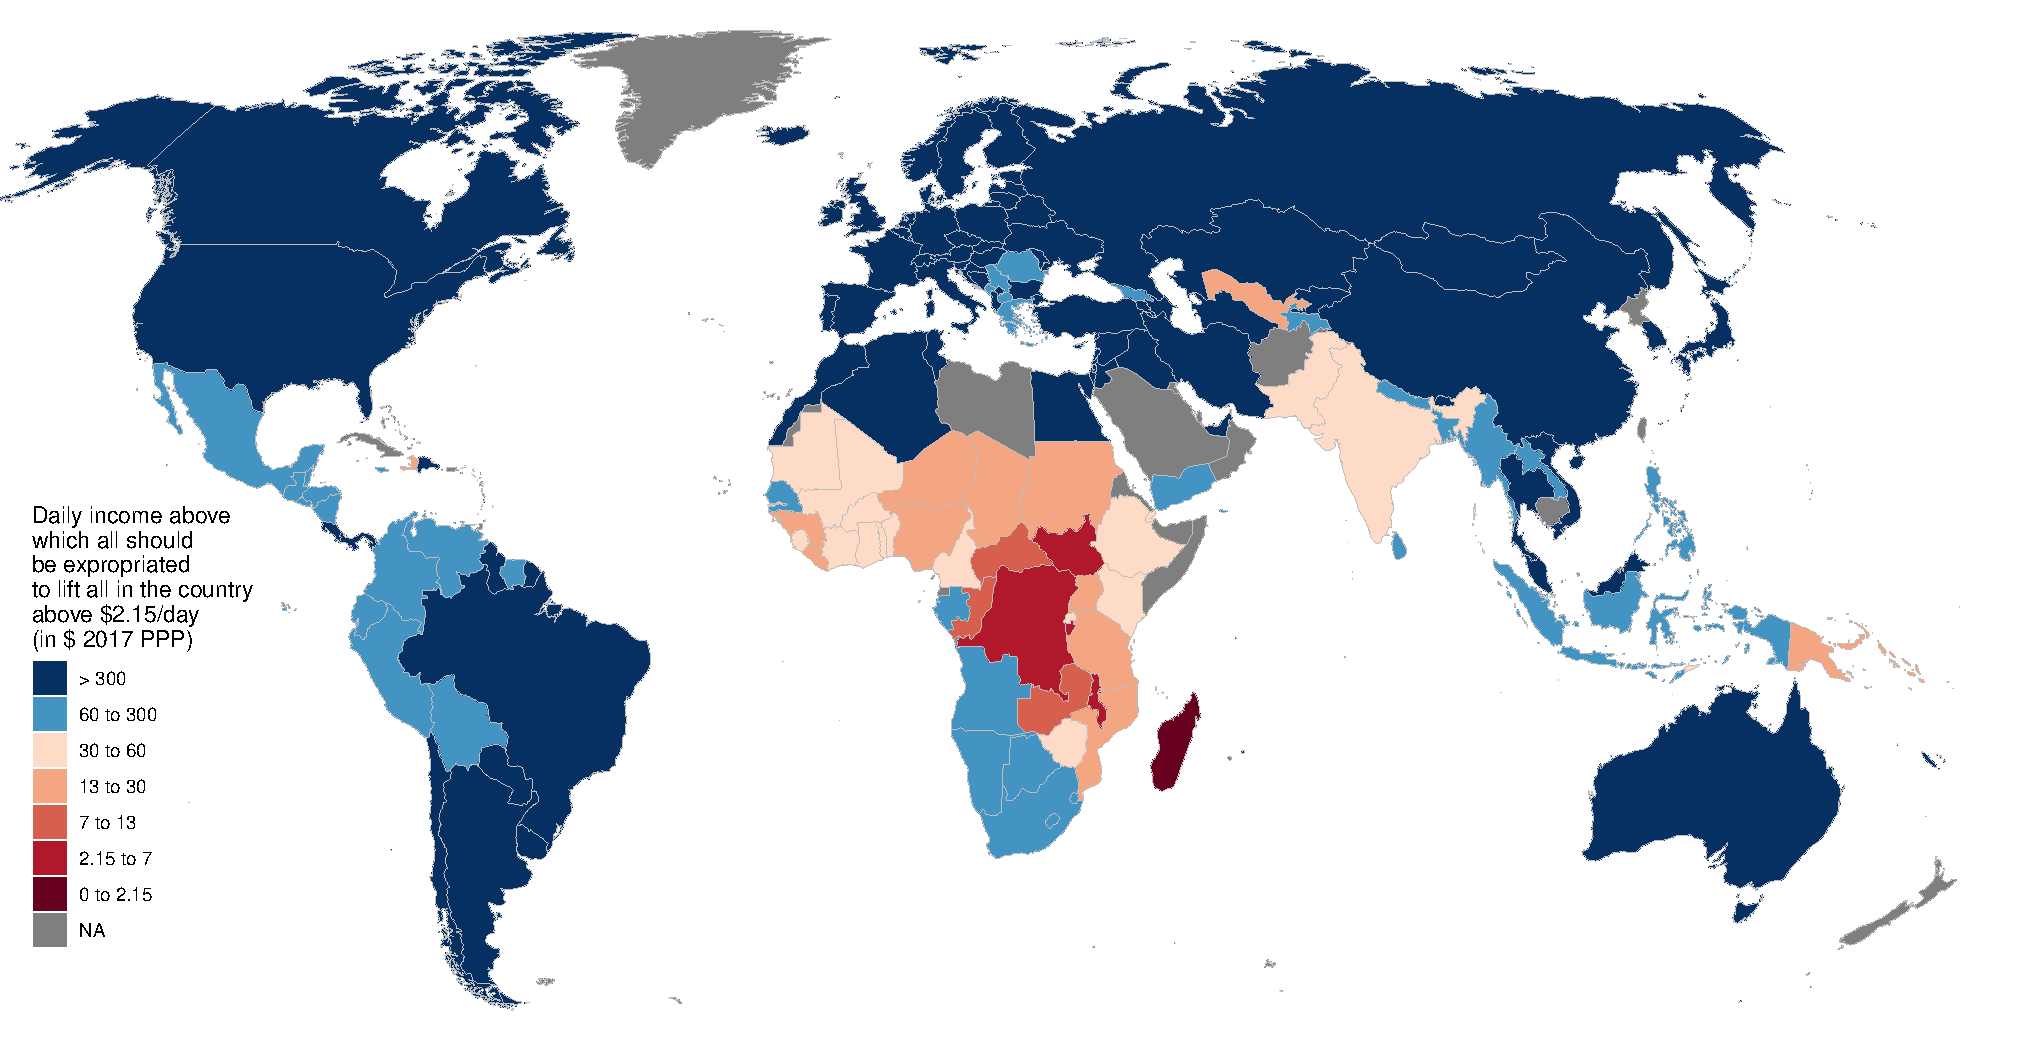
\includegraphics[width=\textwidth]
  {../figures/y_expropriated_2_average.pdf}}
\end{figure} 

In most of the paper, I focus on the definition of extreme poverty employed in the first SDG. However, the \$2.15 threshold has been criticized for inaccurately measuring poverty.\cite{woodward_redefining_2010,deaton_price_2010} % TODO? cite also edward_ethical_2006, pritchett_who_2006
First, this poverty line %is too low to procure just a healthy diet, it is 
is barely sufficient to satisfy one's caloric requirements and is too low to procure a healthy diet or non-food necessities. 
Second, the PPP adjustments applied to PIP data before computing the poverty rates are based on prices of an average consumption basket rather than on prices of subsistence goods.\cite{sullivan_capitalist_2023} Therefore, the cost of a subsistence diet varies across countries. For instance, it is \$1.44 in Malawi vs. \$4.10 in Kenya (in 2011 PPP \$).\cite{moatsos_global_2016} Buidling on earlier work by Robert Allen that addresses these issues,\cite{allen_absolute_2017} Michail Moatsos computes a country-specific poverty line. This basic consumption (or \textit{BCS}) poverty line corresponds to the local price of the cheapest diet that meets caloric and protein requirements, completed with a ration of fat, sugar, and basic non-food requirements.\cite{moatsos_global_2016,moatsos_global_2021,sullivan_capitalist_2023} This alternative measure indicates that poverty % destitution? % On definitions of poverty, cite: Woodward & Abdallah (10) - no data but based on infant mortality rate, Pritchett (06) - 15$ based on HIC poverty lines, Edward (06) - 7$ based on kink in relation between GDP and life expectancy
is more prevalent than the official poverty line suggests. Despite missing data in many countries (including India and the D.R.C.), 14 countries have an average consumption level below this basic consumption poverty line in 2030 in the 3\% growth scenario. These countries (which include e.g. Nigeria) do not have sufficient domestic resources to lift their population above the BCS poverty line, equal to \$4.35/day in median, even after extreme internal redistribution. 
% - Even worse when considering Moatsos' BCS line

BCL found that 62 countries could not eradicate severe poverty (defined as \$$_\text{2005}$2/day) with an antipoverty cap at \$$_\text{2005}$13/day, while 27 could not even do so with a cap at \$$_\text{2005}$2/day. 
Their findings cannot be exactly reproduced with the revised PIP data, as the switch from 2005 to 2017 PPPs has altered not only the level but also the distribution of incomes (for the same reason, the results of BCL and Ravallion cannot be compared). 
When I replicate the computations of BCL (with their survey years but after scaling the original thresholds into 2017 PPPs by a factor $2.15/1.25 = 1.72$), I find that 52 (resp. 30) 
countries could not eradicate severe poverty with a cap at \$22.36/day (resp. \$3.44/day). 
In other words, the revision of PIP data resulted in an apparent enrichment. 
Looking ahead, in our baseline scenario with 3\% growth, we find that in 2030, 34 (resp. 6) 
countries will not be able to eradicate severe poverty with a cap at \$22.36/day (resp. \$3.44/day).

\subsection{Antipoverty taxes}

\begin{figure}[b!]
  \caption[Anti-extreme-poverty tax above \$6.85/day in 2030 after 3\% growth.]{Linear tax rate above \$6.85/day eradicating extreme poverty (in \%). In this idealized policy, all tax revenue is transferred to the extreme poor and lift them at \$2.15/day, assuming away distorsions, and after a yearly growth of 3\% over 2022--2030. 
  }\label{fig:antipoverty_tax_7}
  \makebox[\textwidth][c]{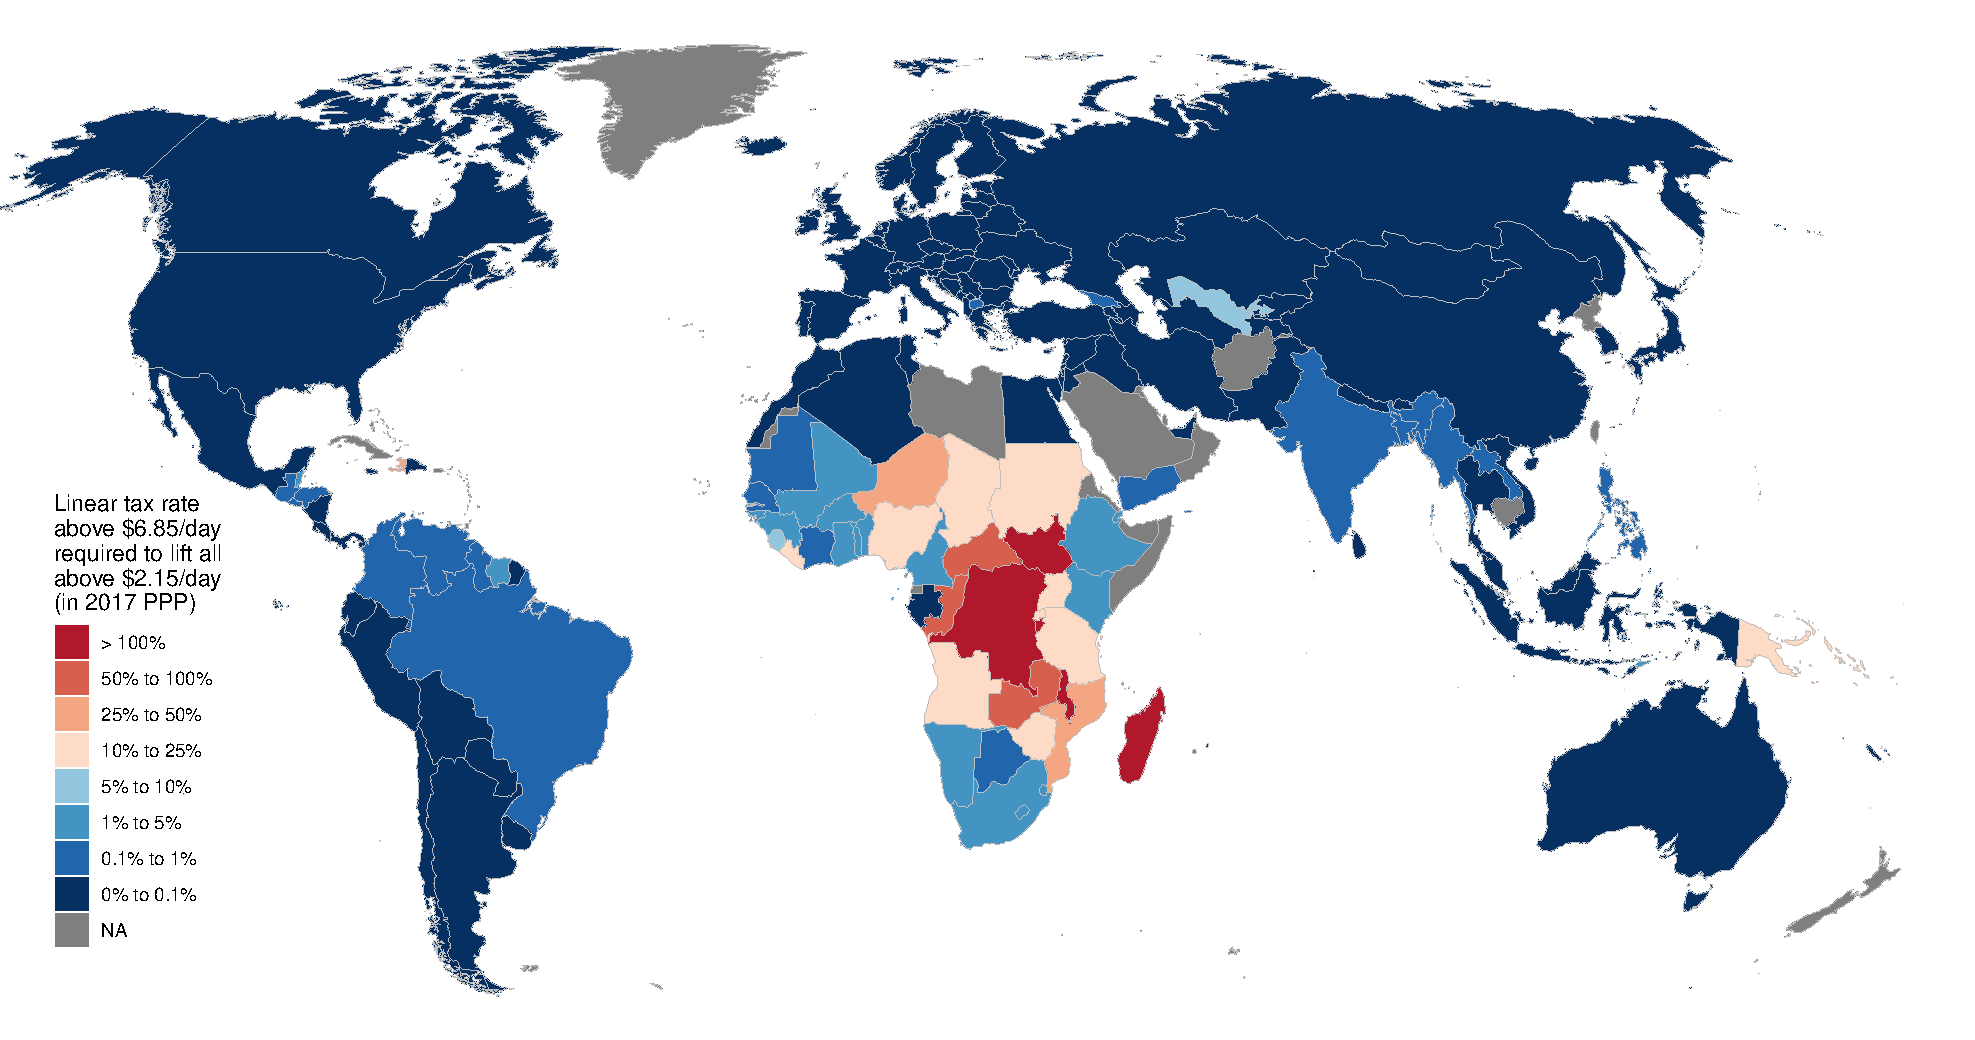
\includegraphics[width=\textwidth]
  {../figures/antipoverty_2_tax_7_average.pdf}}
\end{figure}

Figure \ref{fig:antipoverty_tax_7} presents the (additional) tax rate above \$6.85/day required to generate enough revenues to close the domestic extreme poverty gap, in the baseline scenario of 
3\% growth. The threshold of \$6.85/day is defined by the World Bank and corresponds to an ``acute'' poverty line which can be understood as the consumption level that can sustain a minimally decent life.\cite{hickel_is_2019,kikstra_decent_2021} In contrast, the extreme poverty line of \$2.15/day corresponds to the consumption per capita below which one is undernourished.\cite{allen_absolute_2017} 

Consistently with the previous findings, taxing income at a 100\% rate above \$6.85/day would not generate enough revenues to eliminate extreme poverty in the five poorest countries. In Nigeria, closing the extreme poverty gap would require taxing the ``non-acutely-poor'' at a marginal rate of 20\%. 
On average over Sub-Saharan Africa, the anti-extreme-poverty tax would be 49\%, and 70\% in low-income countries (defined by the World Bank as countries with a GNI per capita below \$1,135 per year). Yet, imposing such a large tax burden on any income above just \$6.85/day seems unrealistic. 

\begin{figure}[b!]
  \caption[Anti-extreme-poverty tax above \$18.15/day in 2030 after 3\% growth.]{Linear tax rate above \$18.15/day eradicating extreme poverty (in \%). In this idealized policy, all tax revenue is transferred to the extreme poor and lift them at \$2.15/day, assuming away distorsions, and after a yearly growth of 7\% over 2022--2030.
  }\label{fig:antipoverty_tax_18}
  \makebox[\textwidth][c]{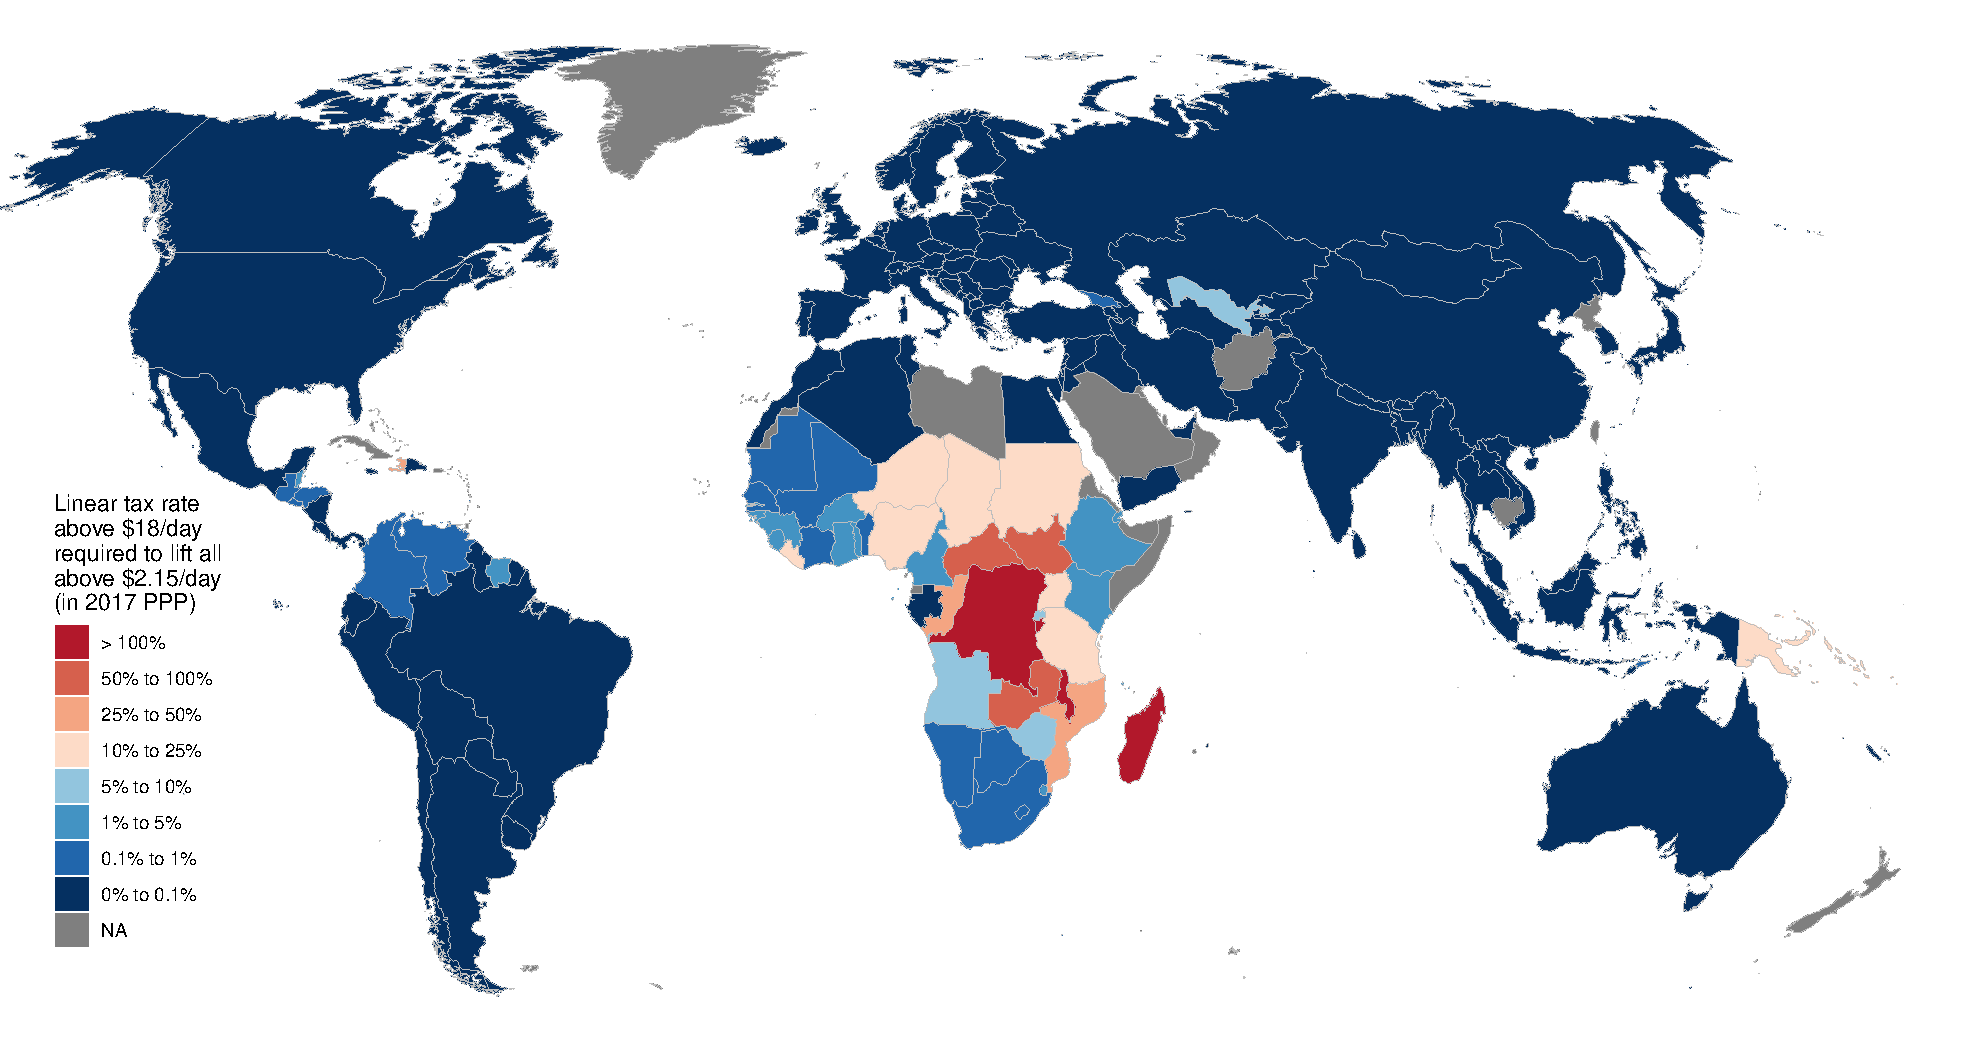
\includegraphics[width=\textwidth]
  {../figures/antipoverty_2_tax_18_very_optimistic.pdf}}
\end{figure}

Figure \ref{fig:antipoverty_tax_18} presents the anti-extreme-poverty tax on incomes above \$18.15/day, in a very optimistic scenario of 7\% growth. The threshold of \$18.15/day per person corresponds to the U.S. federal poverty line for a family of four and represents a more realistic threshold above which taxes could be increased in the Global South. The anti-extreme-poverty tax rates on the ``non-poor'' % non-US-poor?
in this 7\% growth scenario are comparable to the rates on the non-acutely-poor in the baseline scenario. In India, the required tax rate would be 10\% % 9.7\%
% in the scenario of 7\% growth, and 36\% if growth until 2030 replicates the 2014--2019 trend (5.5\% per year). 
in the scenario with 7\% growth until 2030, 36\% with 5.5\% growth (the country's 2014--2019 trend), and unachievable (at 156\%) with 3\% growth. %if growth until 2030 replicates the 2014--2019 trend (5.5\% per year). 
With sustained growth, the contribution required of the Indian non-poor seems large but possible. % significant but not unreasonable. 
Therefore, India seems able to eliminate extreme poverty by 2030 with its domestic resources. The same thing cannot be said of Sub-Saharan Africa. %Therefore, lower-middle income countries like India seem able to eliminate extreme poverty by 2030 with its domestic resources. The same thing cannot be said of low-income countries, most of them in Sub-Saharan Africa. %

% By default, 6\% (7?) growth starting in 2023 
% - Tax rate to eradicate poverty: above 7, 18: Figure 2

\subsection{The credible potential of domestic redistribution}

A final way of approaching the issue is to set a tax schedule, compute how much revenues it would generate in each country, and estimate the income floor that these revenues could finance (by topping up the incomes of the poorest to the income floor). As I have already explored extreme redistributive policies, I analyse here a more reasonable tax schedule. Namely, I consider a 10\% marginal tax rate on income above \$6.85/day. Although the tax base may be too wide (affecting people on the verge of acute poverty) % taxation threshold may be too low 
and the tax rate too low for top incomes, 
this simple tax schedule seems to correctly reflect the fiscal capacity of governments. Note that the value of the income floor depends on the whole income distribution: the top of the distribution determines the revenues that can be generated; and the bottom dictates the cost of raising low incomes up to a given floor. 

% - would have worked well if it had been 7\% since 2016
\begin{figure}[b!]
  \caption[Income floor of 10\% tax above \$6.85/day in 2030 after 3\% growth.]{Income floor that can be funded with a 10\% marginal tax on income above \$6.85/day (in 2017 PPP \$/day). In this idealized policy, all tax revenue is transferred to the poorest and lift them at the income floor, assuming away distorsions, and after a yearly growth of 3\% over 2022--2030. 
  }\label{fig:demogrant_7__10}
  \makebox[\textwidth][c]{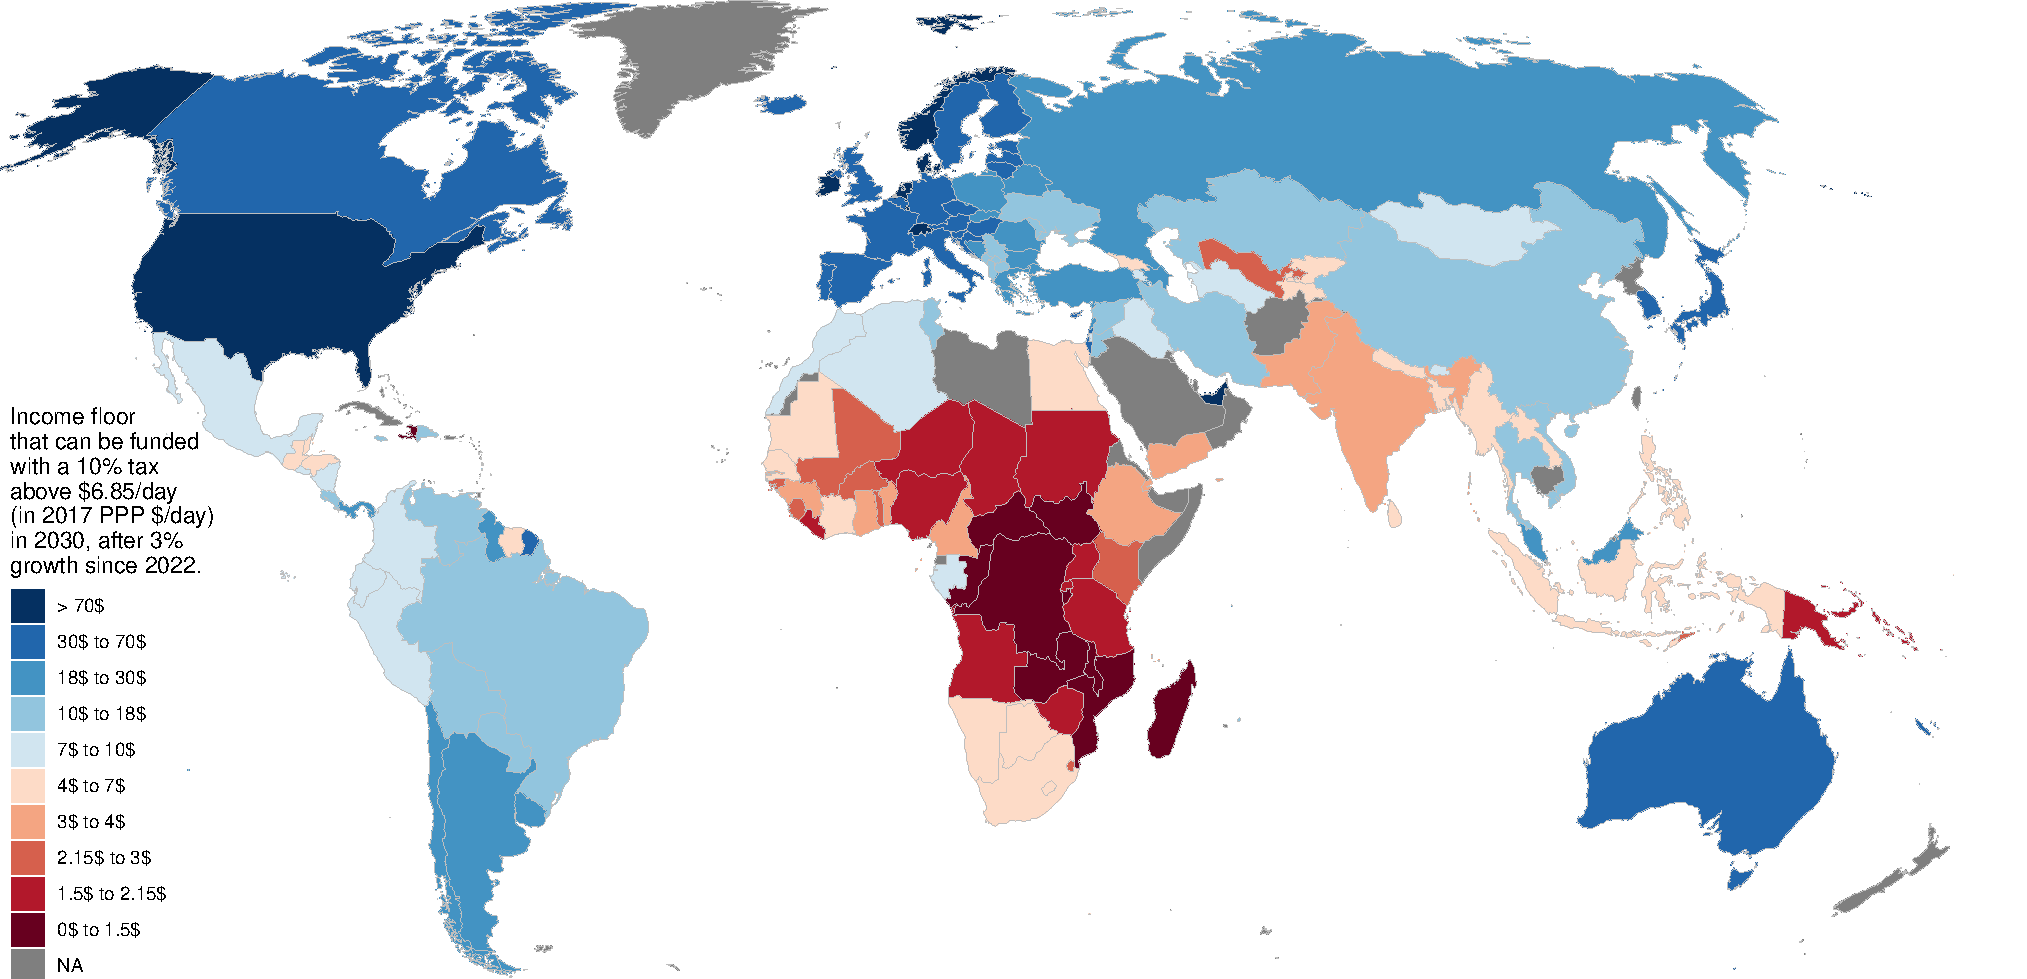
\includegraphics[width=\textwidth]
  {../figures/demogrant_7__10.pdf}}
\end{figure}

Figure \ref{fig:demogrant_7__10} presents the income floor that can funded in 2030 with our simple tax in a 3\% growth scenario. While the number of countries unable to eradicate extreme poverty through this tax totals 23, a figure akin to the count of low-income countries at 27, a mere 13 countries fall into both categories.
%Although there are about as many countries that cannot close the extreme poverty gap with this tax (23) as there are low-income countries (27), only 13 countries fall into both of these groups. 
For example, while Ethiopia (a low-income country) can finance an income floor of \$3.08/day, Nigeria (classified as a lower-middle-income country) can only finance a floor of \$1.83/day. 

Even in a scenario with 7\% growth from 2023 onwards, 10 countries have an income floor below \$2.15 in 2030. Note that the picture does not significantly change when adjusting top incomes so that aggregate consumption matches national accounts:\cite{deaton_measuring_2005,prydz_disparities_2022} 
8 countries are still unable to close the extreme poverty gap despite very optimistic growth in this robustness check. In contrast, if the 7\% growth had started in 2016 (as the SDGs were set up), the 10\% tax would have been sufficient to eliminate extreme poverty in all countries except in Madagascar, where a tax of 23\% would have been required.

At least two of the SDGs spell out how the elimination of extreme poverty could be funded. % https://sdgs.un.org/2030agenda
First, the target 8.1 aims for ``at least 7 per cent gross domestic product growth per annum in the least developed countries''. As we have seen, a sustained high growth since 2016 would have permitted the least developed countries to eliminate extreme poverty through the mobilization of their domestic resources. However, high growth has never materialized in these countries. 
Second, the target 17.2 calls for ``Developed countries to implement fully their official development assistance commitments, including the commitment by many developed countries to achieve the target of 0.7 per cent of ODA/GNI to developing countries and 0.15 to 0.20 per cent of ODA/GNI to least developed countries'' (LDCs). Foreign aid falls short of both the overall target (at 0.37\% of developed countries' GNI) and the LDCs' target (at 0.06\%). While just four countries are meeting their commitments (Luxembourg, Sweden, Norway, and Germany), the U.S. only allocates 0.23\% of its GNI to foreign aid.\cite{oecd_oda_2023} The global extreme poverty gap (0.17\% of global real GDP) is a bit lower than the shortfall of foreign aid relative to the target (0.2\% of global nominal GDP), suggesting that extreme poverty could be eradicated if developed countries respected their commitment. % OECD (high-income) countries represent 59% (61%) of the world nominal GDP, so shortfall of aid is 0.34*0.59=0.2% of global GDP in nominal. https://data.worldbank.org/indicator/NY.GDP.MKTP.CD
However, to meet the broader SDGs and ``end poverty in all its forms'', the 0.7\% target would not suffice and international solidarity should be significantly strenghtened. %global redistribution would need to be significantly increased. % TODO? system change => already in conclusion
% shorten: take out this paragraph

\subsection{The potential of global redistribution} % TODO? solidarity?

In this section, we highlight the potential of globally redistributive policies to close the global poverty gap in 2030 in the baseline scenario of 3\% growth. %The policies described are idealized and should be understood as proxies for any action of international solidarity or system change that would bring about an equivalent transfer of resources. TODO? put back?
% The wealth tax simulator of the World Inequality Lab\cite{chancel_world_2022} shows that a global 1.05\% marginal tax on wealth above \$100 million would collect 0.2\% of the global GDP, enough to close the extreme poverty gap. Alternativaly, one can collect the same amount (around \$200 billion per year) with a 2.8\% tax above \$1 billion or with a 0.47\% tax above \$5 million.

If applied to the global level, the tax of the previous section would bring the global Gini from .62 down to .51 and finance an income floor at \$8.6/day, thereby closing the \$6.85/day poverty gap. By comparison, applied at the national level, it would only bring the global Gini down to .59 and reduce the poverty gap from 4.5\% to 3.7\% of global income. 

To close the \textit{extreme} poverty gap, a 1.2\% marginal tax % TODO? rate?
above 100\$/day (i.e. \$36,500/year) would suffice. %raise revenues equal to the 2030 . 
Such a tax would result in 3.4\% of global income being transferred from the rich to the extreme poor, but would only involve 0.14\% of global income being transferred from one country to another. 
With contributions of up to 0.4\% of a country's income (in the U.S.), aggregate consumption would increase by more than 10\% in 9 countries. 
%Low-income countries would receive 3\% of their consumption (and up to 11\% in the D.R.C. or 36\% in Madagascar) 
% while the U.S. would contribute 0.4\% of its consumption.
% To raise 1\% of the world GDP and finance an \$4/day income floor, the rate should be increased to 8\%. 
%However, to end poverty in all its forms, about 5\% of global consumption should be redirected to the poor, enough to raise the global income floor to \$7.15/day. This would require higher tax rates, for example 25\% above 100\$/day and 75\% above 200\$/day. 
% These rates are expressed on top of the current tax system and apply to post-tax income. For example, the last tax schedule would leave unaffected the 96\% of the world population with a post-tax income per capita below \$3,000/month, reduce by 10\% the post-tax income at \$5,000/month, and reduce it  by 37\% at \$10,000/month. 

% TODO! I can't use the HFCE-rescaled results if I attribute all extra income to the top 1% => Add orders of magnitude for global wealth tax + in NS version, keep only the wealth tax (bc HFCE entirely attributed to >100$/d leads to net losses in HMICs and wo HFCE losses are too high in HICs) 
In reality, the global tax rates required to eradicate poverty may well be lower than just indicated, because our calculations used the raw PIP data instead of converting them to nominal terms and rescaling them to national accounts. Once I rescale the data to national accounts, (which are more accurate in high-income countries), 
a mild 0.3\% marginal tax above \$100/day suffices to close the extreme poverty gap. Raising that rate to 10\% would collect 3.4\% of the world income, enough to finance a global income floor of \$7/day and end poverty in all its forms. 
These rates are expressed on top of the current tax system and apply to post-tax income. For example, the last tax schedule would leave unaffected the 95\% of the world's population whose per capita after-tax income is less than \$36,500/year, and would reduce the after-tax income of those at \$73,000/year by 5\%. 
% TODO? Use ws instead of w? 

% 6.85 pg: 4.5% (less in nominal); 2.15 pg: .15%
% https://wid.world/world-wealth-tax-simulator/
% 4/6/7/8/9% > 1/20/200M/1/10G => 4.22% (tax = k yield)
% 3/4/5/6/7/8% > 500k/1/20/200M/1/10G => 4.96% (tax = k yield)
% 4/10% > 1/100M => 4.41%
% 2.1% > 1G => 0.15%
% top 1%: 1M

% Although the idea of an internationally redistributive tax may seem far-fetched, 
Although internationally redistributive taxes have yet to take off, the proposal of a global wealth tax is gaining momentum.\cite{piketty_brief_2022} A 2\% tax on individual net wealth above \$1 billion would raise \$214 billion a year, slightly more than the global extreme poverty gap.\cite{tax_observatory_global_2024} Moreover, a global tax on the wealthiest 1\% can raise enough revenues to close the global acute poverty gap and lift everyone above \$6.85/day. For example, the \href{https://wid.world/world-wealth-tax-simulator}{WID wealth tax simulator} shows that a tax consisting of a 4\% marginal rate above \$1 million and 10\% above \$100 million would raise 4.4\% of the global GDP. More generally, a global tax on millionaires designed to be revenue-maximing in the long-run has the potential to finance the eradication of acute poverty. 

In a nutshell, whereas poverty alleviation cannot be achieved rapidly without international solidarity, it can be financed by reasonable contributions from the global top 1\%.
% - One example of global redistribution (incl. largest recipients/contributors)
% x Inequality indicators BAU / national / global redistr: Table 2

\section{Discussion} 

To paraphrase the UN, ``as things stand, the world is not on track to end poverty by 2030.''\cite{un_sustainable_2022} I have shown that the only prospect for low-income countries to eliminate extreme poverty on their own is the combination of strong growth, ambitious policies of social programs and internal redistribution, and time. 
With record growth and profound government committment, China has officially eradicated extreme poverty in 2021. The D.R.C. is poorer now than China in 1990, % https://data.worldbank.org/indicator/SI.POV.DDAY?locations=CD-CN-AE, https://data.worldbank.org/indicator/NY.GDP.PCAP.PP.KD?locations=ET-CN-CD
so even if it reproduces the Chinese miracle, it cannot eradicate extreme poverty on its own before 2055. 
In contrast, international solidarity could end poverty more quickly and at a much lower welfare cost. In this paper, I have illustrated the magnitude of the required transfer of resources with idealized international taxes, but in reality this could take other forms such as a systemic change in the rules or structures of the world economy. 
To be fair, this paper only presents the orders of magnitude of global inequality. %Poverty is multidimensional and t
In practice, structural factors (like wars or corruption) that sustain poverty %, corruption, or deficient administrative capacity). 
can also hamper the effectiveness of international action. %research can help design % uncovering?
While concrete policy proposals have the potential % If... are the way
to mobilize international solidarity,\cite{fabre_international_2023} research can help design effective policies to distribute resources to the poorest.
% “As things stand, the world is not on track to end poverty by 2030,” (UN, 22)
% # World Bank (2022): "It became clear that the global goal of ending extreme poverty by 2030 would not be achieved."
% Paper shows that extreme poverty will not be eradicated in 2030 unless international transfers. 
% Even in the longer term, only strong growth + strong internal redistribution + time can allow countries to eliminate extreme poverty on their own (cite the time that China took: DRC lower GDPpc and higher extreme poverty rate than China in 90). 
% In contrast, international transfers might solve the issue more quickly and at a much lower welfare cost. 
% However, this paper only arithmetics, poverty is multidimensional and sustained structural factors (wars, corruption, deficient administrative capacity). These factors can hamper the effectiveness of international transfers. More research needed to study concrete policies on how to distribute resources to the poorest.

% \begin{methods}  % WPcomment
  \begin{small} % NCCcomment
%Put methods in here.  If you are going to subsection it, use \subsection commands.  Methods section should be less than 800 words and if it is less than 200 words, it can be incorporated into the main text.

% \section*{\normalsize Methods}\label{sec:methods} % NCCcomment
% \addcontentsline{toc}{section}{\nameref{sec:methods}}


% \subsection*{\small Data quality.} % WPcomment 
% \paragraph{\small Data quality.} % NCCcomment 


\section*{\normalsize Data and code availability}

All data and code of as well as figures of the paper are available on \href{https://github.com/bixiou/domestic_poverty_eradication}{github.com/bixiou/domestic\_poverty\_eradication}. 

% \end{methods} % WPcomment
\end{small}  % NCCcomment

% \bibliographystyle{naturemag_noURL} % nature class works only with style naturemag or naturemag_noURL, and naturemag bugs if there are certain URLs (like .pdf). Also, nature class only works with \cite, not \citet or \citep.  % WPcomment
\renewcommand{\url}[1]{\href{#1}{Link}} % NCCcomment
\bibliographystyle{plainnaturl_clean} % NCCcomment
\bibliography{poverty}
% \input{app} 

% WPcomment
%% Here is the endmatter stuff: Supplementary Info, etc.
%% Use \item's to separate, default label is "Acknowledgements"
% \begin{addendum} % 177 words
\begin{itemize}
 \item[Acknowledgments] I am grateful to Michalis Moatsos for his help in using his data. I thank Lidia Ceriani for providing her data. I thank Thomas Goumont and Elise Thai for research assistance. 
 \item[Competing Interests] I declare that I also serve as president of Global Redistribution Advocates.
\item[JEL codes] D63, I32, P16.
\item[Keywords]  Poverty gap, Sustainable Development Goals, Domestic resource mobilization, Redistribution, Fiscal capacity, Extreme poverty.
 \item[Correspondence] Correspondence and requests for materials
should be addressed to Adrien Fabre~(email: adrien.fabre@cnrs.fr).\end{itemize}
% \end{addendum}

\clearpage
\listoftables
\listoffigures

\appendix % NCCcomment
\renewcommand{\thetable}{A\arabic{table}}
\renewcommand{\thefigure}{A\arabic{figure}}
\setcounter{figure}{0}
\setcounter{table}{0}

\clearpage
\section{Appendix}
\subsection{Additional figures}

Many more figures (with varying poverty lines, taxation thresholds, growth scenarios, etc.) are available on \href{https://github.com/bixiou/domestic_poverty_eradication/tree/main/figures}{github.com/bixiou/domestic\_poverty\_eradication}. Also, any custom figure can be easily produced using this code.

% Main text figures:
% y_expropriated_2_average
% antipoverty_2_tax_7_average
% antipoverty_2_tax_18_very_optimistic
% demogrant_7__10

% Appendix figures:
% s_antipoverty_2_tax_7_average
% antipoverty_2_tax_7_reg
% antipoverty_2_tax_18_average
% s_antipoverty_2_tax_18_very_optimistic
% antipoverty_4_tax_18_average
% antipoverty_7_tax_18_average
% antipoverty_7_tax_7_average
% demogrant_7__10_very_optimistic
% s_demogrant_7__10

\begin{figure}[!htb]
  \caption[Anti-extreme-poverty tax above \$6.85/day after 3\% growth (HFCE-scaled).]{Linear tax rate above \$6.85/day eradicating extreme poverty (in \%). Data has been rescaled to match HFCE aggregate from national account. In this idealized policy, all tax revenue is transferred to the extreme poor and lift them at \$2.15/day, assuming away distorsions, and after a yearly growth of 3\% over 2022--2030. 
  }\label{fig:s_antipoverty_2_tax_7_average}
  \makebox[\textwidth][c]{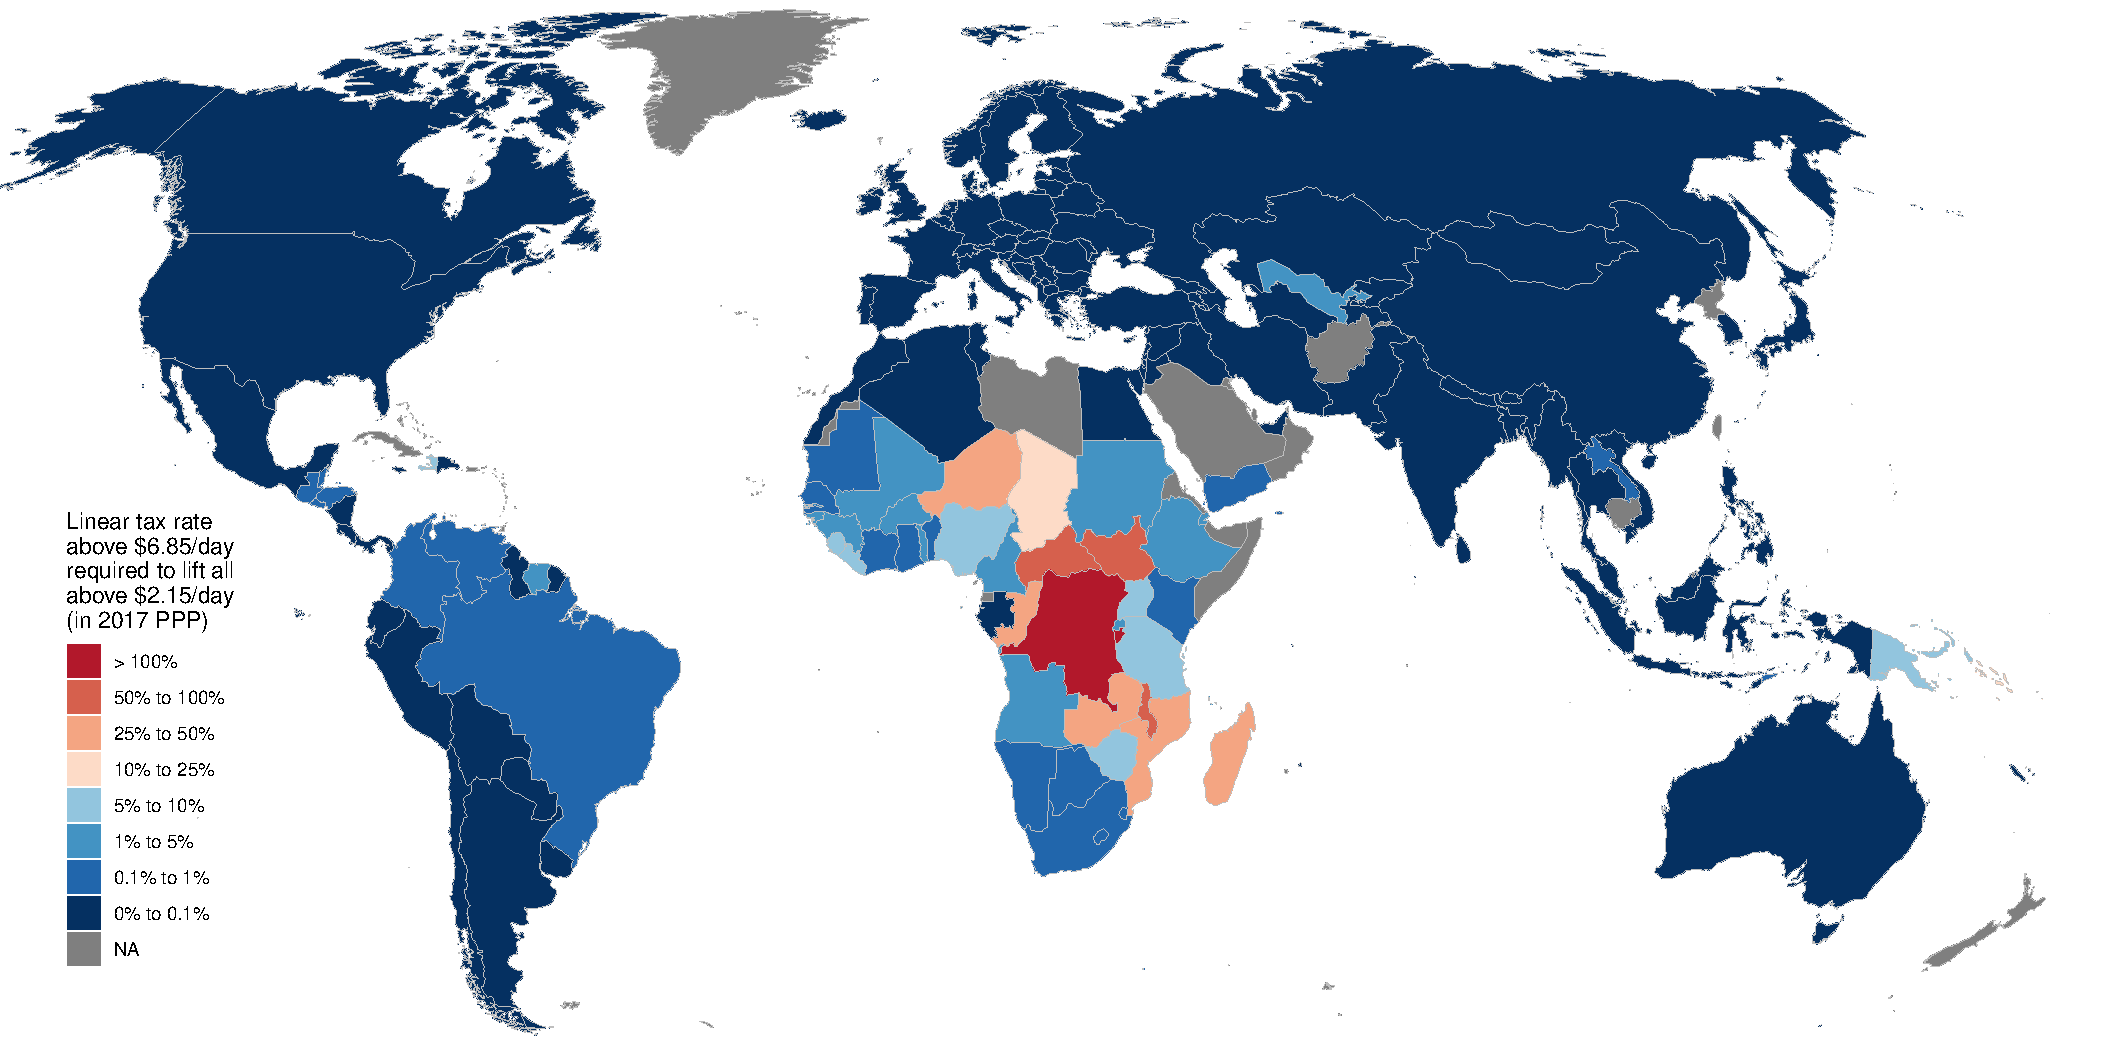
\includegraphics[width=\textwidth]
  {../figures/s_antipoverty_2_tax_7_average.pdf}}
\end{figure}

\begin{figure}[!htb]
  \caption[Anti-extreme-poverty tax above \$6.85/day after 3\% growth (HFCE-scaled).]{Linear tax rate above \$6.85/day eradicating extreme poverty (in \%). In this idealized policy, all tax revenue is transferred to the extreme poor and lift them at \$2.15/day, assuming away distorsions, with growth until 2030 predicted at the country level. 
  }\label{fig:antipoverty_2_tax_7_reg}
  \makebox[\textwidth][c]{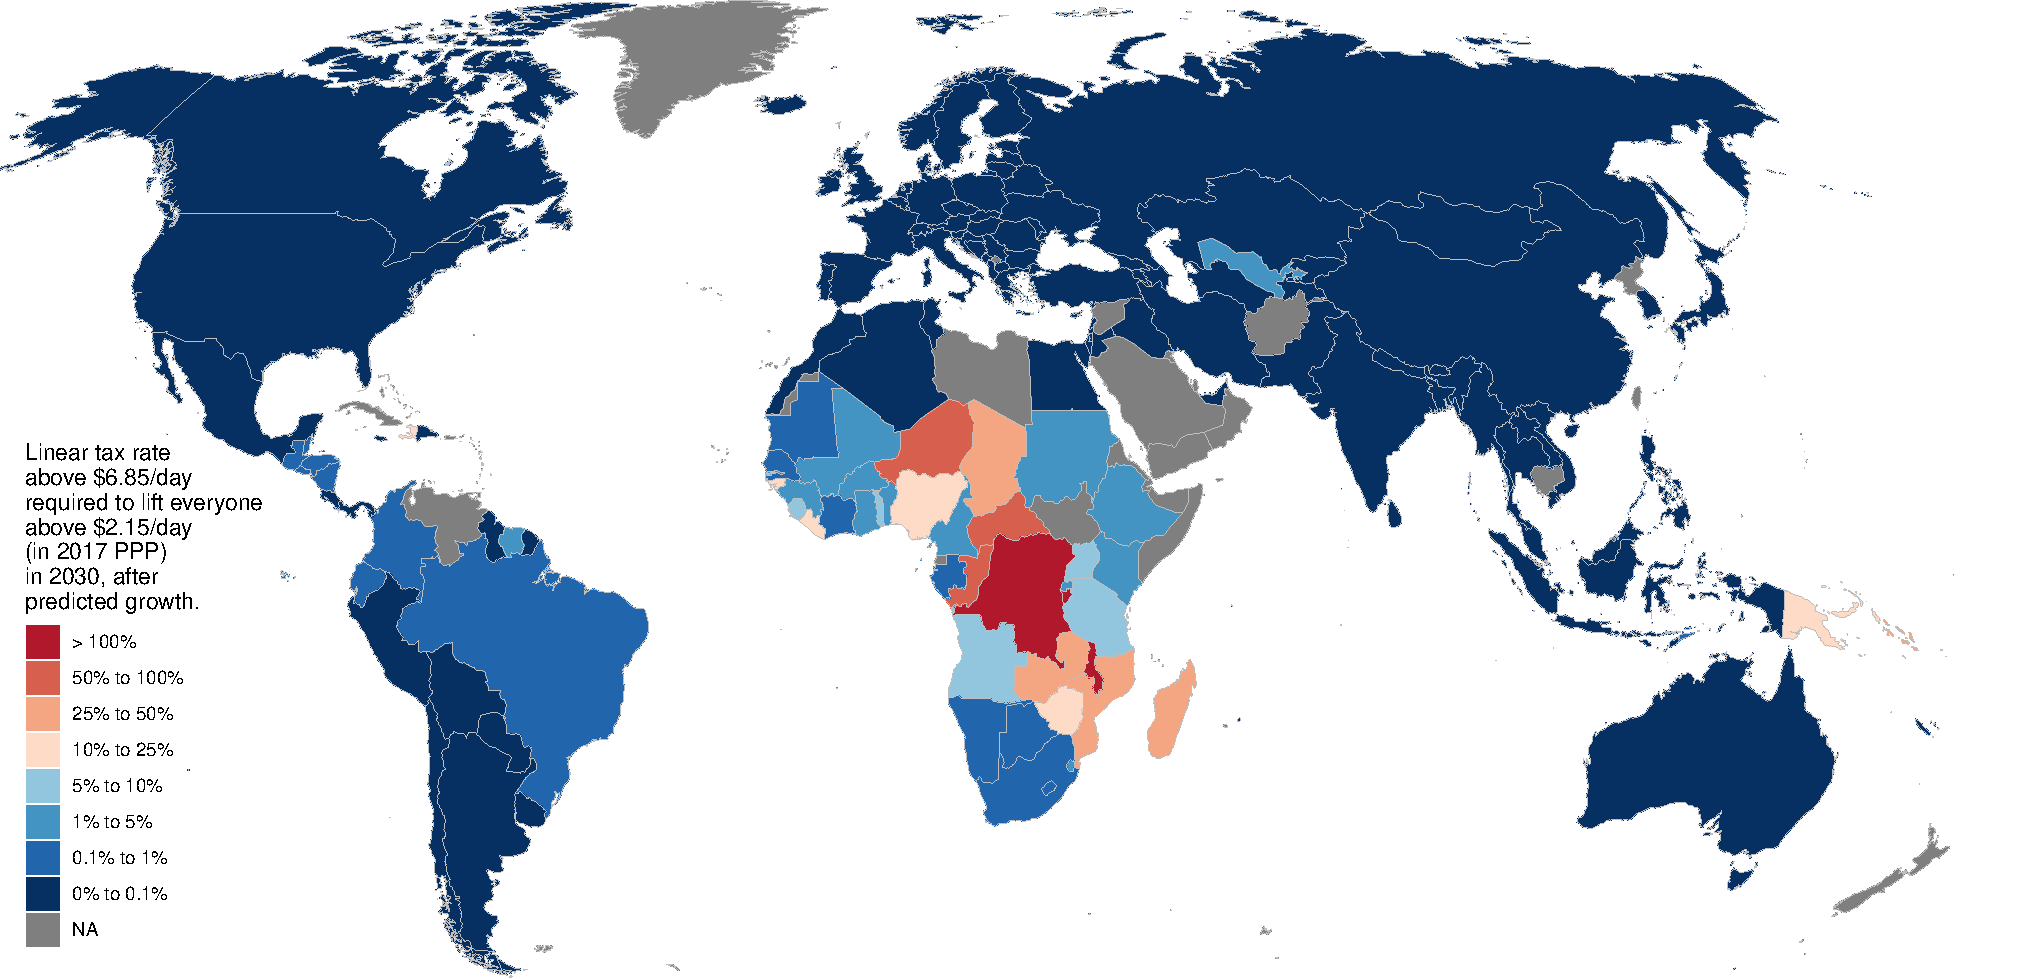
\includegraphics[width=\textwidth]
  {../figures/antipoverty_2_tax_7_reg.pdf}}
\end{figure}

\begin{figure}[!htb]
  \caption[Anti-extreme-poverty tax above \$18.15/day after 3\% growth.]{Linear tax rate above \$18.15/day eradicating extreme poverty (in \%). In this idealized policy, all tax revenue is transferred to the extreme poor and lift them at \$2.15/day, assuming away distorsions, and after a yearly growth of 3\% over 2022--2030. 
  }\label{fig:antipoverty_2_tax_18_average}
  \makebox[\textwidth][c]{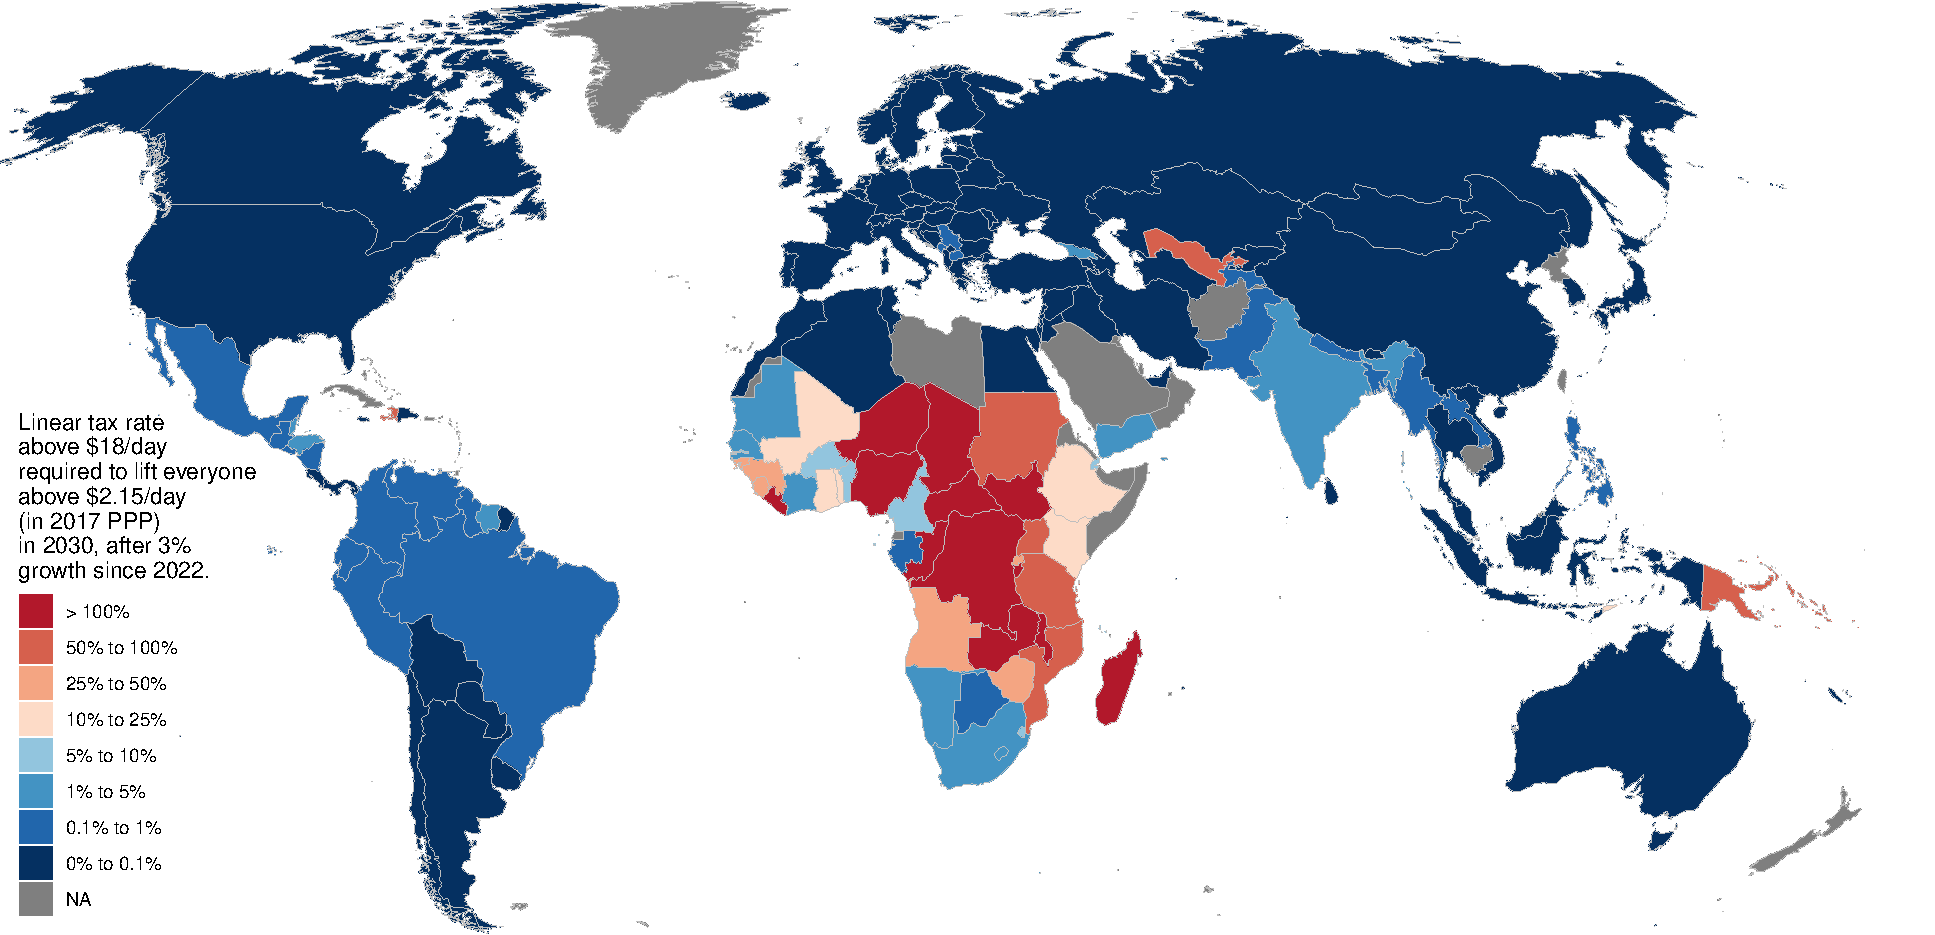
\includegraphics[width=\textwidth]
  {../figures/antipoverty_2_tax_18_average.pdf}}
\end{figure}

\begin{figure}[!htb]
  \caption[Anti-extreme-poverty tax above \$18.15/day after 7\% growth (HFCE-scaled).]{Linear tax rate above \$18.15/day eradicating extreme poverty (in \%). Data has been rescaled to match HFCE aggregate from national account. In this idealized policy, all tax revenue is transferred to the extreme poor and lift them at \$2.15/day, assuming away distorsions, and after a yearly growth of 7\% over 2022--2030. 
  }\label{fig:s_antipoverty_2_tax_18_very_optimistic}
  \makebox[\textwidth][c]{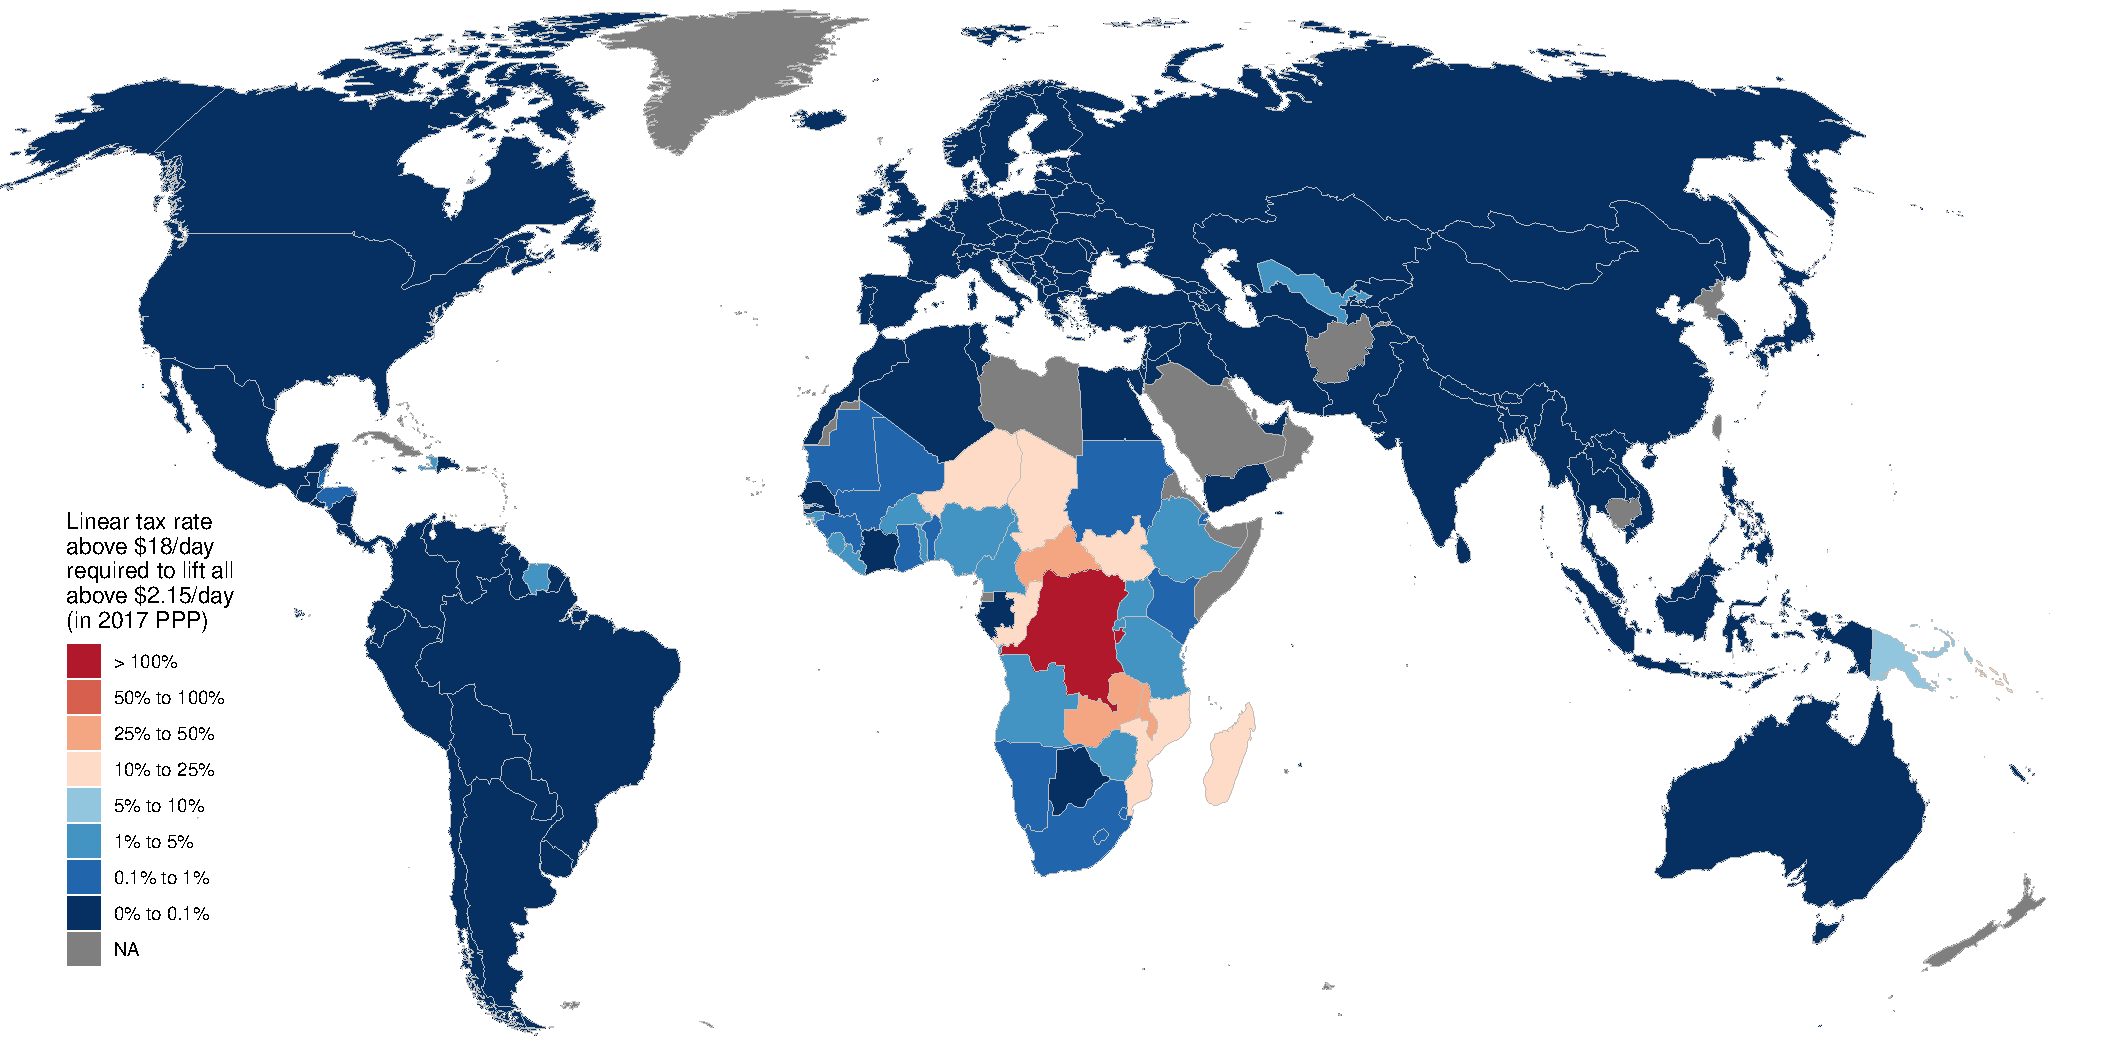
\includegraphics[width=\textwidth]
  {../figures/s_antipoverty_2_tax_18_very_optimistic.pdf}}
\end{figure}

\begin{figure}[!htb]
  \caption[Anti-severe-poverty tax above \$18.15/day after 3\% growth (HFCE-scaled).]{Linear tax rate above \$18.15/day eradicating extreme poverty (in \%). In this idealized policy, all tax revenue is transferred to the extreme poor and lift them at \$3.65/day, assuming away distorsions, and after a yearly growth of 3\% over 2022--2030. 
  }\label{fig:antipoverty_4_tax_18_average}
  \makebox[\textwidth][c]{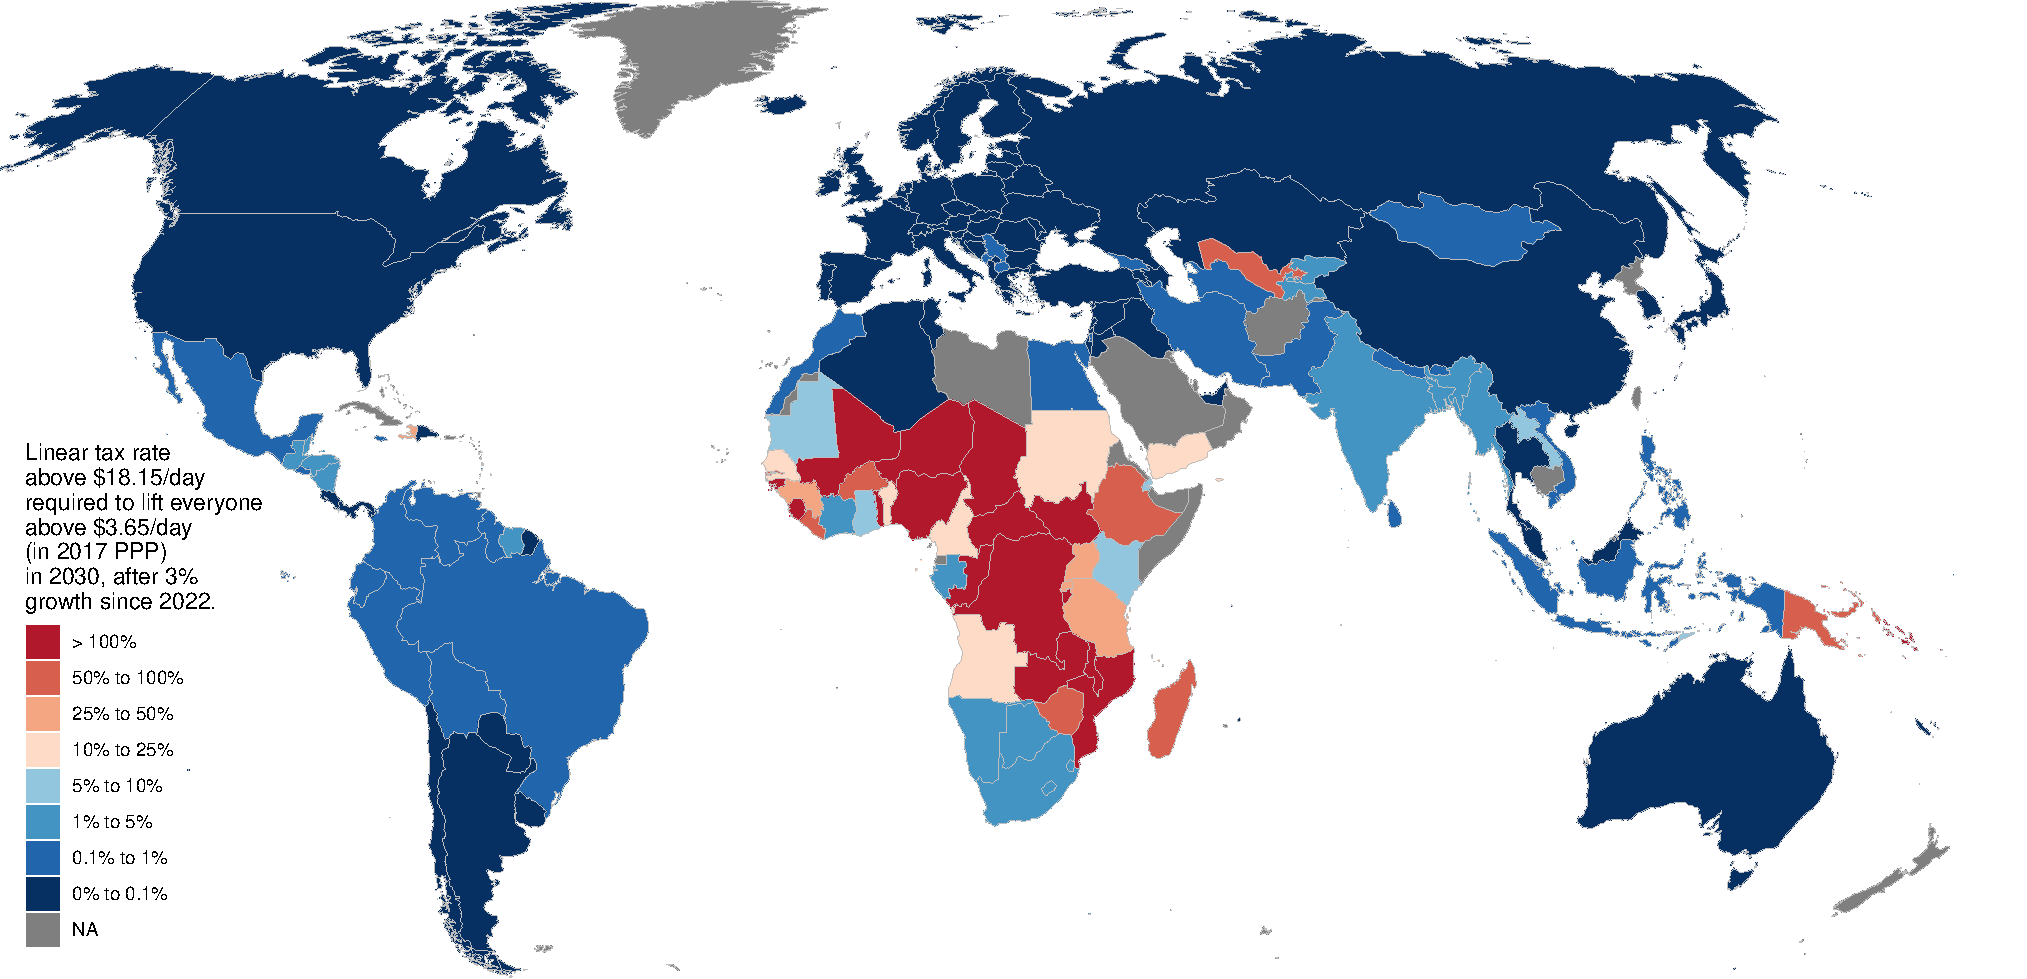
\includegraphics[width=\textwidth]
  {../figures/antipoverty_4_tax_18_average.pdf}}
\end{figure}

\begin{figure}[!htb]
  \caption[Anti-acute-poverty tax above \$18.15/day after 3\% growth (HFCE-scaled).]{Linear tax rate above \$18.15/day eradicating extreme poverty (in \%). In this idealized policy, all tax revenue is transferred to the extreme poor and lift them at \$6.85/day, assuming away distorsions, and after a yearly growth of 3\% over 2022--2030. 
  }\label{fig:antipoverty_7_tax_18_average}
  \makebox[\textwidth][c]{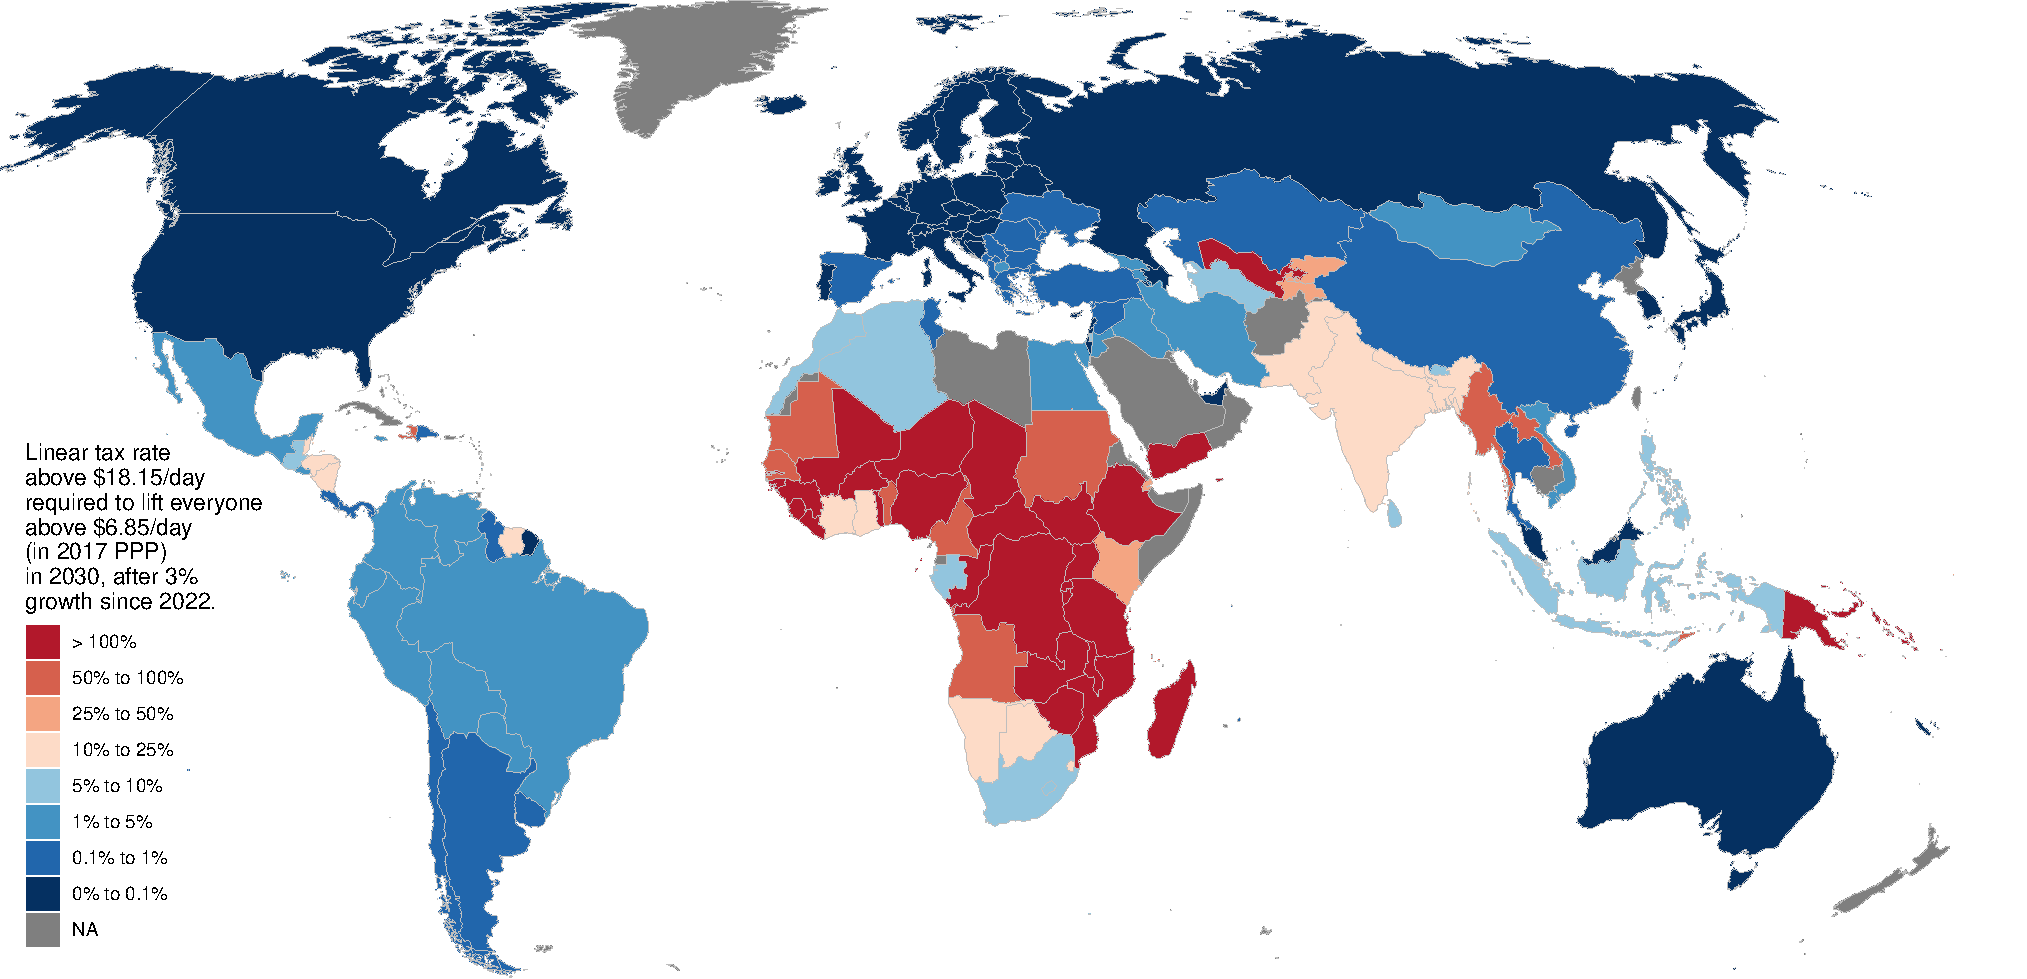
\includegraphics[width=\textwidth]
  {../figures/antipoverty_7_tax_18_average.pdf}}
\end{figure}

\begin{figure}[!htb]
  \caption[Anti-acute-poverty tax above \$6.85/day after 3\% growth (HFCE-scaled).]{Linear tax rate above \$6.85/day eradicating extreme poverty (in \%). In this idealized policy, all tax revenue is transferred to the extreme poor and lift them at \$6.85/day, assuming away distorsions, and after a yearly growth of 3\% over 2022--2030. 
  }\label{fig:antipoverty_7_tax_7_average}
  \makebox[\textwidth][c]{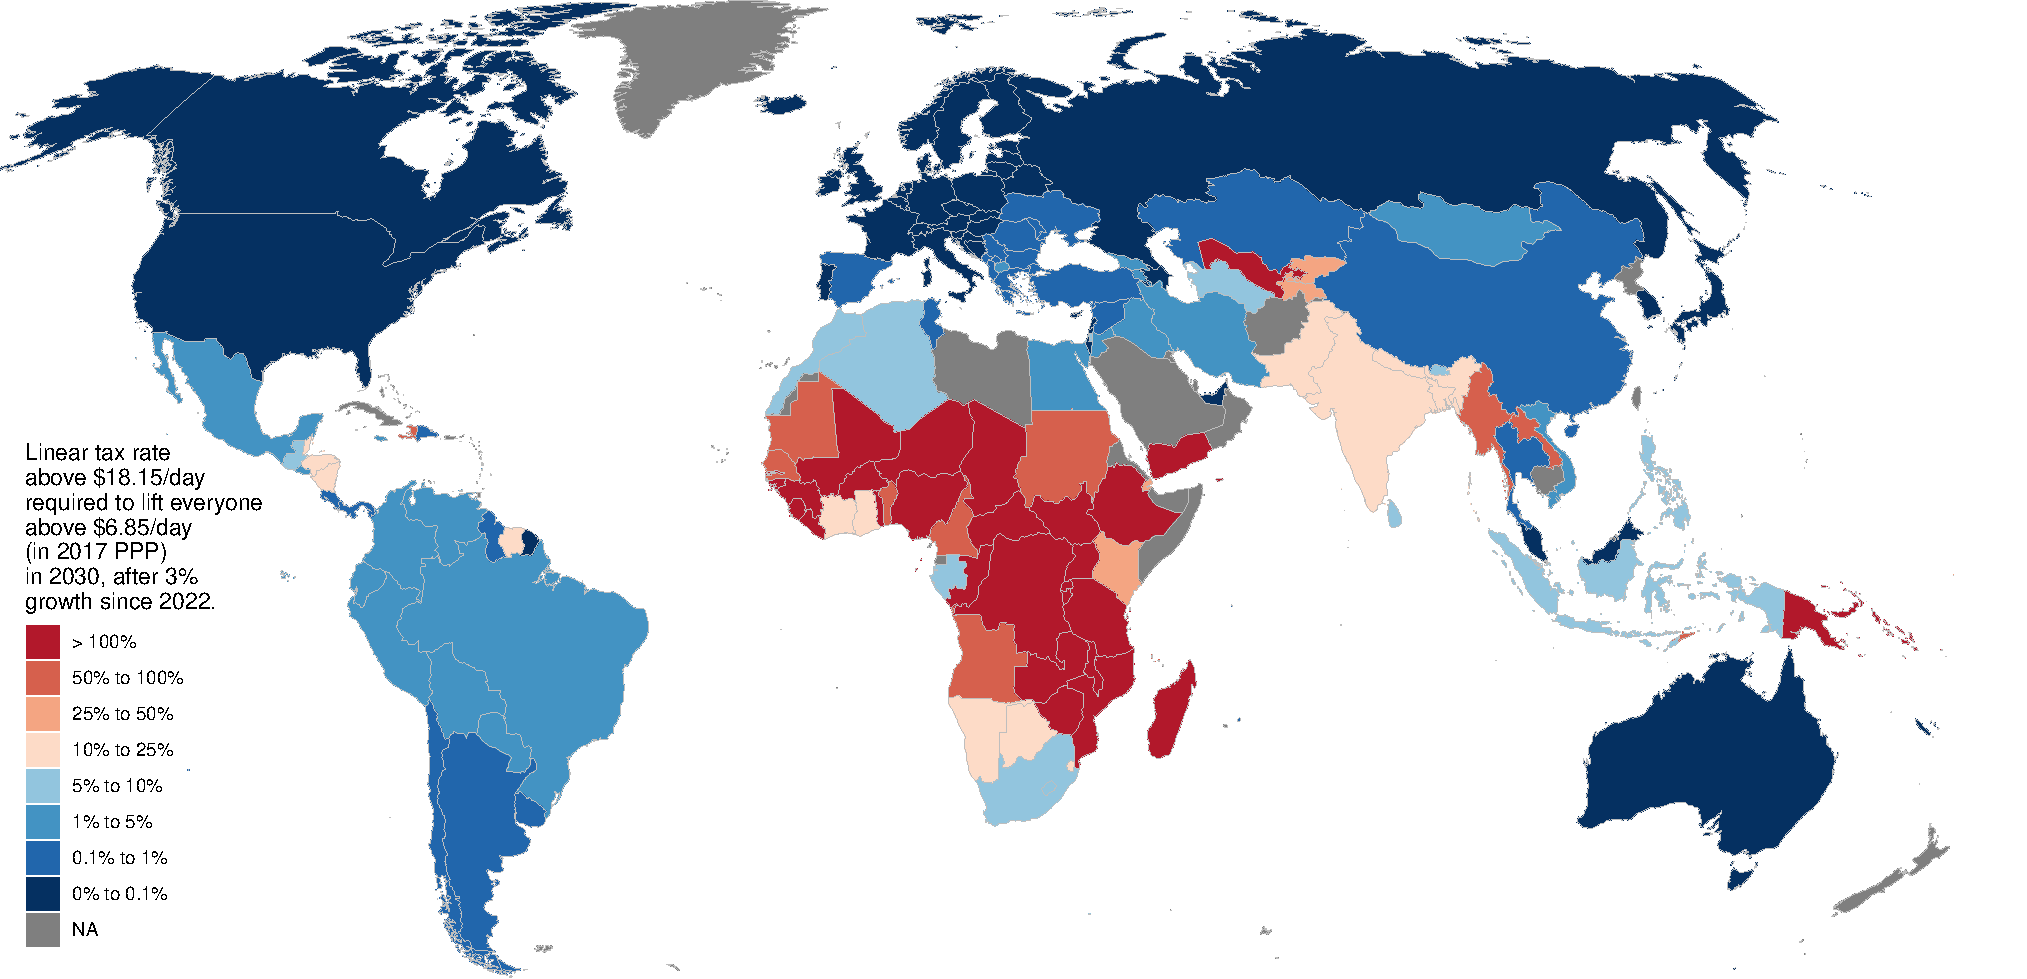
\includegraphics[width=\textwidth]
  {../figures/antipoverty_7_tax_7_average.pdf}}
\end{figure}

\begin{figure}[!htb]
  \caption[Income floor of 10\% tax above \$6.85/day after 7\% growth.]{Income floor that can be funded with a 10\% marginal tax on income above \$6.85/day (in 2017 PPP \$/day). In this idealized policy, all tax revenue is transferred to the poorest and lift them at the income floor, assuming away distorsions, and after a yearly growth of 7\% over 2022--2030. 
  }\label{fig:demogrant_7__10_very_optimistic}
  \makebox[\textwidth][c]{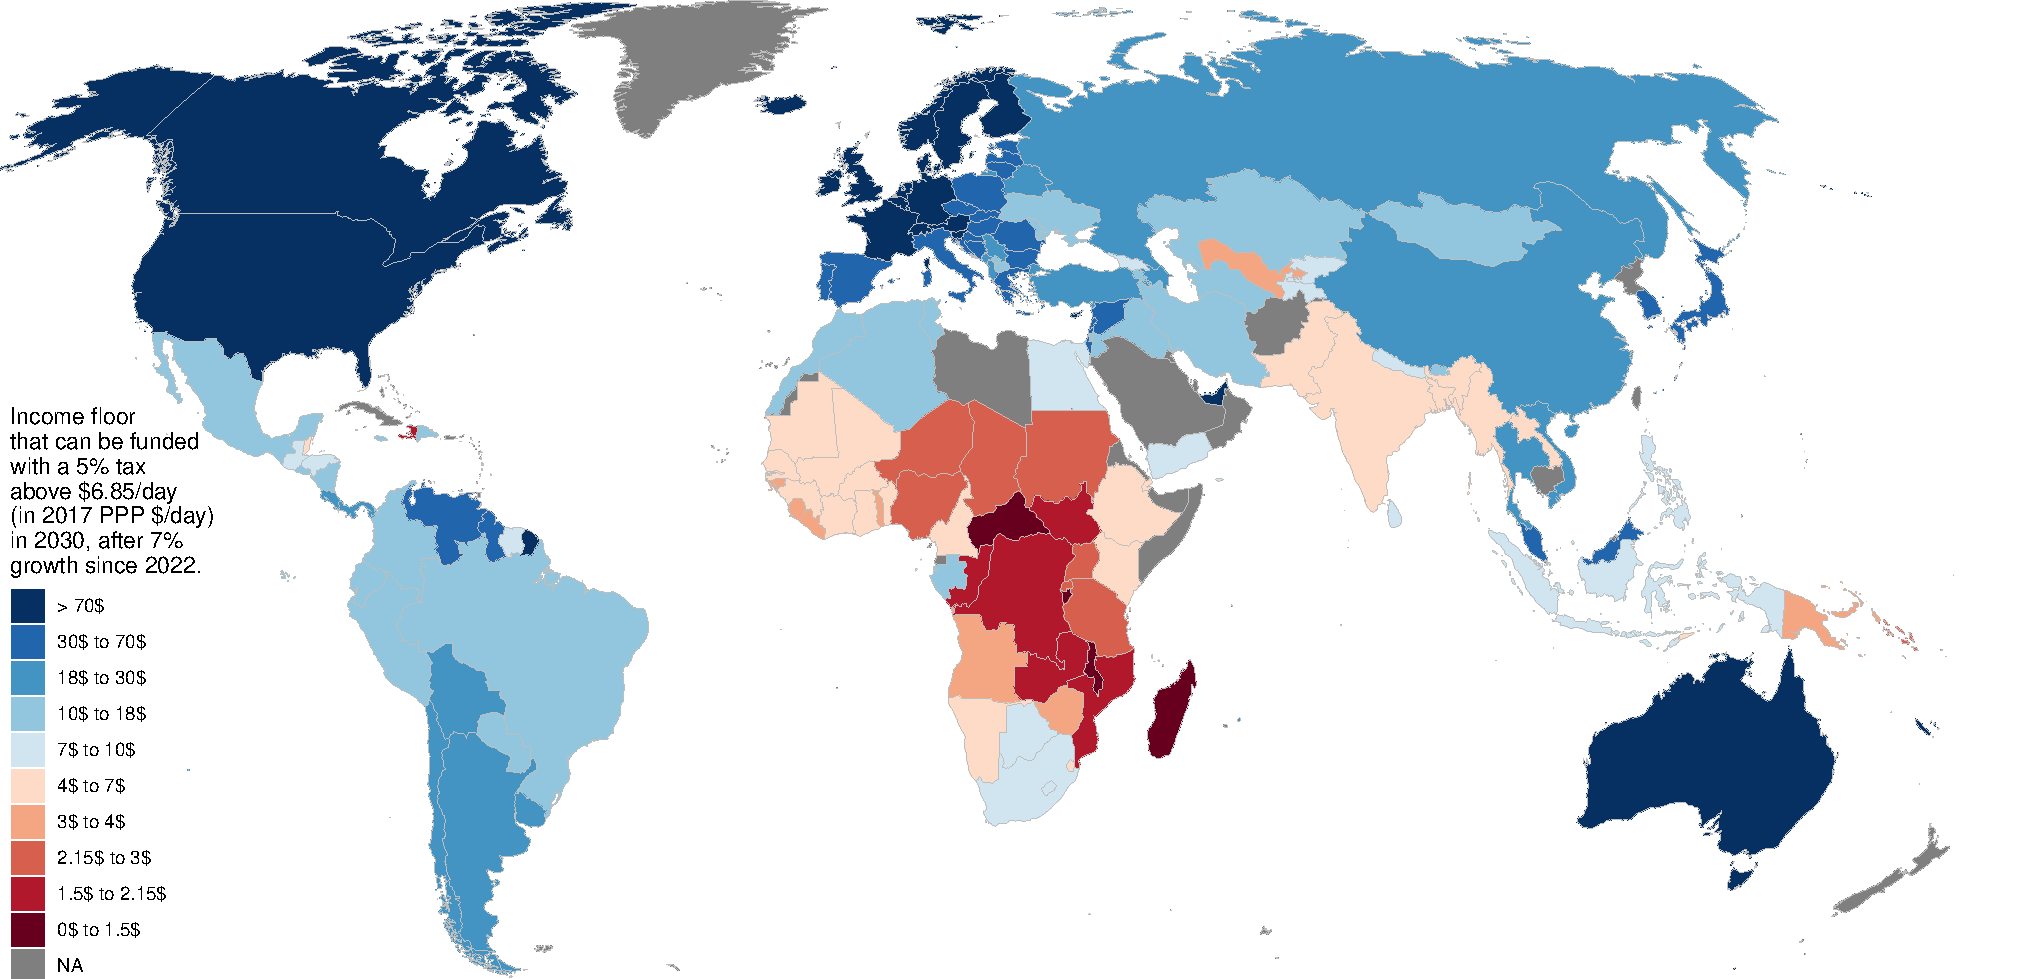
\includegraphics[width=\textwidth]
  {../figures/demogrant_7__10_very_optimistic.pdf}}
\end{figure}

\FloatBarrier
\begin{figure}[!htb]
  \caption[Income floor of 10\% tax above \$6.85/day after 3\% growth (HFCE-scaled).]{Income floor that can be funded with a 10\% marginal tax on income above \$6.85/day (in 2017 PPP \$/day). Data has been rescaled to match HFCE aggregate from national account. In this idealized policy, all tax revenue is transferred to the poorest and lift them at the income floor, assuming away distorsions, and after a yearly growth of 3\% over 2022--2030. 
  }\label{fig:s_demogrant_7__10}
  \makebox[\textwidth][c]{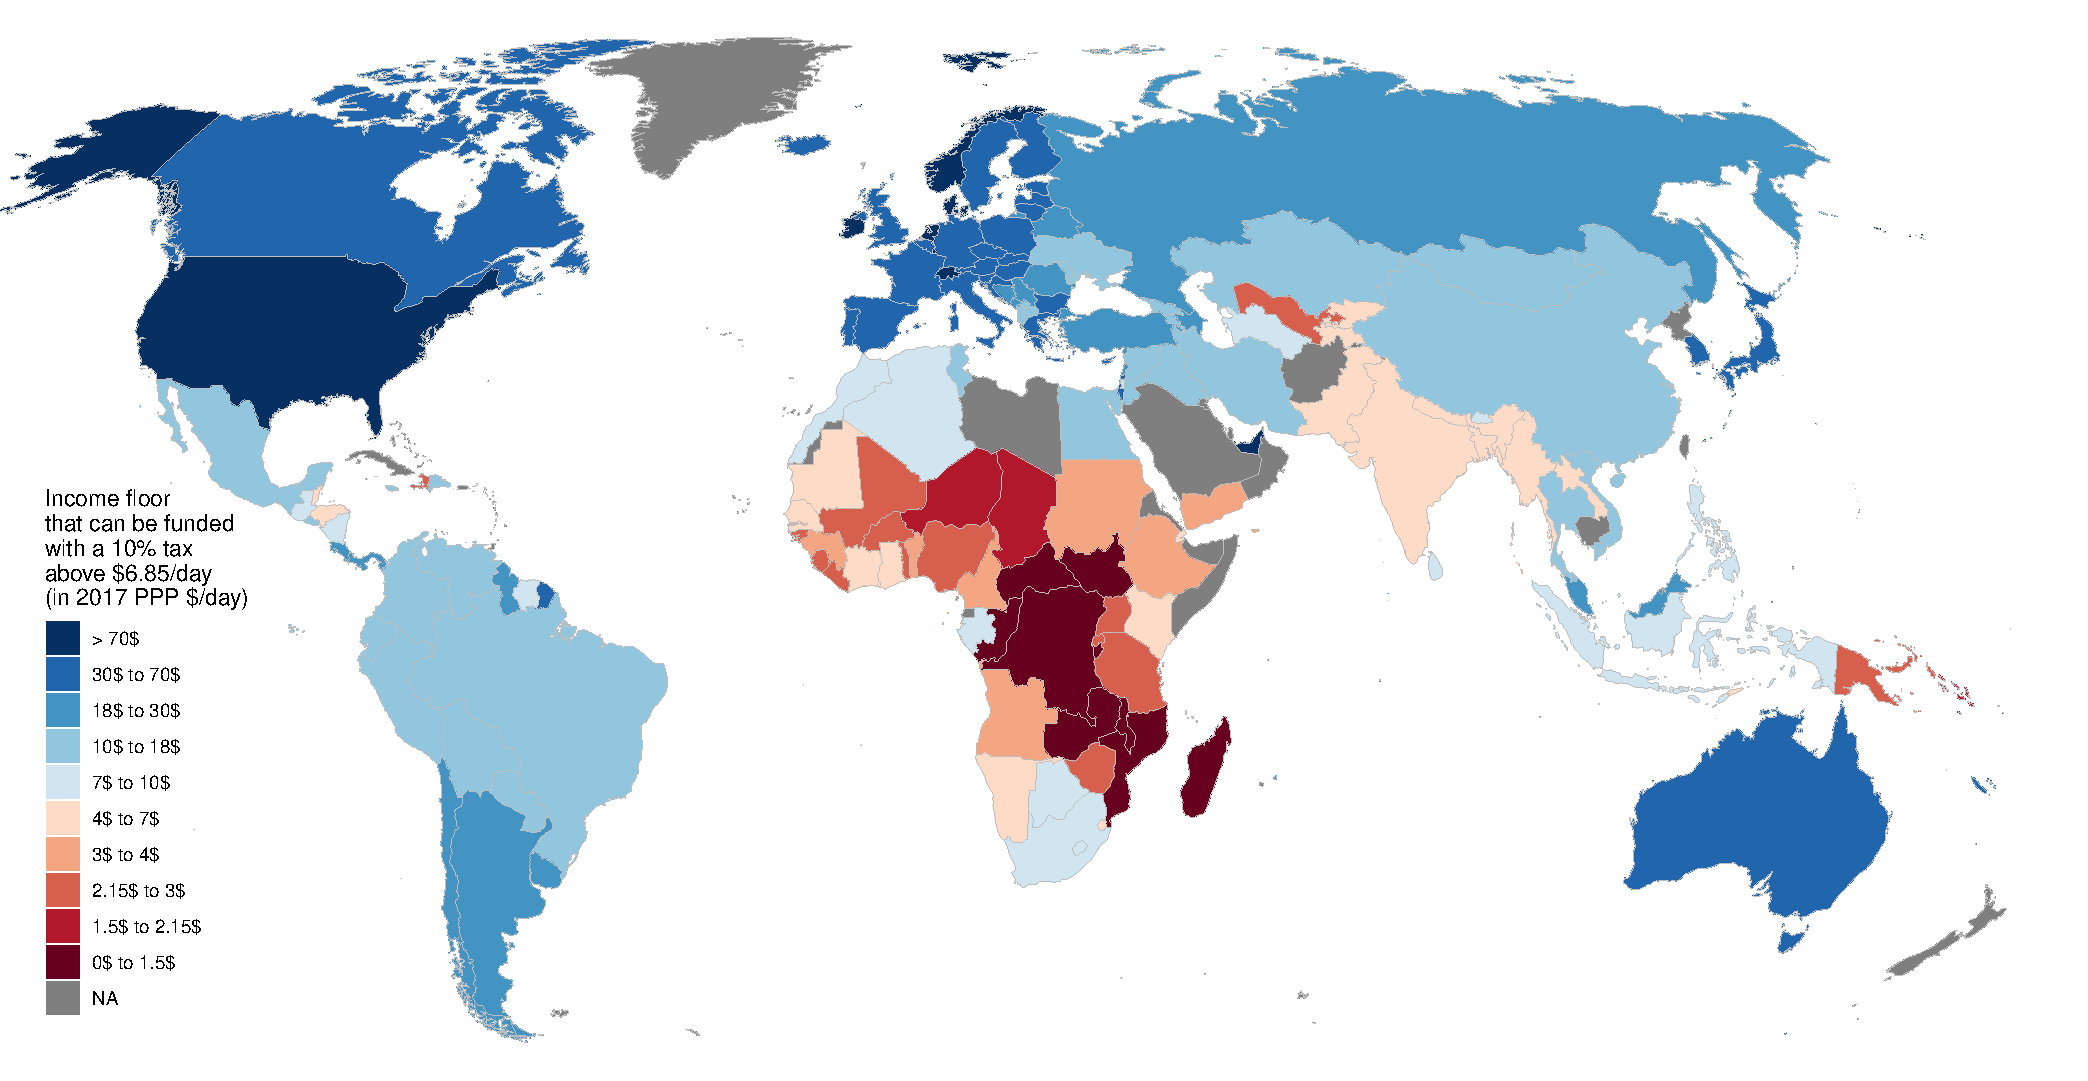
\includegraphics[width=\textwidth]
  {../figures/s_demogrant_7__10.pdf}}
\end{figure}

\subsection{Additional tables}
\begin{table}[b]

\caption[Mean income in different scenarios, survey years and HFCE rescaling factor.]{\label{tab:tax}Mean income for major countries in various years and growth scenarios, survey years and factor used to rescale incomes to national accounts (in countries with HFCE to survey ratio above 1).}
\makebox[\textwidth][c]{
\begin{tabular}[t]{lccccccccc}
\toprule  & Year & \multicolumn{6}{c}{Mean consumption/income (in \$/day)} & BCL & HFCE to  \\ 
 Indicator & of & year of & 2022 & \multicolumn{4}{c}{2030 estimate} & survey & survey \\ 
 & Survey & survey & est. & 3\% & 7\% & Projection & Trend & year & ratio \\ 
\midrule
World & 2018 & 17.2 & 18.6 & 23.6 & 32.3 & 22.9 & 23.4 & 2009 & 1.42\\
Low-Income Countries & 2015 & 3.9 & 4.1 & 5.7 & 9.2 & 4.7 & 5.1 & 2009 & 1.12\\
Sub-Saharan Africa & 2016 & 4.2 & 4.3 & 5.5 & 7.4 & 5.1 & 5.0 & 2009 & 1.34\\
\midrule Algeria & 2011 & 9.2 & 9.3 & 11.8 & 16.0 & 10.4 & 9.4 & 1995 & 1.36\\
Angola & 2018 & 5.5 & 4.7 & 6.0 & 8.1 & 5.2 & 4.7 & 2009 & 1.71\\
Argentina & 2021 & 24.8 & 25.8 & 32.7 & 44.4 & 29.8 & 25.8 & 2010 & 1.43\\
Bangladesh & 2016 & 4.5 & 6.1 & 7.7 & 10.5 & 8.0 & 9.6 & 2010 & 1.90\\
Brazil & 2021 & 19.2 & 19.6 & 24.9 & 33.8 & 22.2 & 19.6 & 2009 & 1.26\\
Canada & 2018 & 65.7 & 65.7 & 83.3 & 112.9 & 73.2 & 69.3 & NA & 1.10\\
China & 2019 & 14.9 & 17.0 & 21.5 & 29.1 & 25.8 & 27.4 & 2009 & 1.15\\
Colombia & 2021 & 14.2 & 15.1 & 19.1 & 26.0 & 17.9 & 16.3 & 2010 & 1.89\\
D.R. Congo & 2012 & 2.0 & 2.6 & 3.2 & 4.4 & 3.0 & 2.8 & 2005 & 0.91\\
Egypt & 2019 & 6.8 & 7.3 & 9.3 & 12.6 & 8.6 & 9.1 & 2008 & 3.64\\
Ethiopia & 2015 & 3.7 & 5.1 & 6.4 & 8.7 & 7.0 & 8.1 & 2011 & 0.91\\
France & 2020 & 57.4 & 62.5 & 79.2 & 107.5 & 69.6 & 69.4 & NA & 1.04\\
Germany & 2019 & 65.9 & 65.5 & 83.0 & 112.5 & 73.7 & 71.8 & NA & 1.10\\
India & 2019 & 5.3 & 5.6 & 7.1 & 9.7 & 7.3 & 8.6 & 2010 & 2.19\\
Indonesia & 2022 & 7.9 & 7.9 & 10.0 & 13.6 & 9.8 & 10.8 & NA & 2.21\\
Iraq & 2012 & 11.3 & 11.2 & 14.2 & 19.3 & 12.6 & 13.5 & 2007 & 1.36\\
Italy & 2020 & 49.8 & 55.7 & 70.6 & 95.8 & 60.9 & 62.2 & NA & 1.13\\
Japan & 2013 & 49.8 & 52.4 & 66.3 & 90.0 & 58.3 & 56.5 & NA & 1.13\\
Kenya & 2015 & 4.2 & 5.0 & 6.3 & 8.6 & 5.8 & 6.1 & 2005 & 1.99\\
Mexico & 2020 & 14.0 & 14.9 & 18.9 & 25.6 & 16.6 & 16.1 & 2010 & 2.17\\
Morocco & 2013 & 10.6 & 11.6 & 14.7 & 19.9 & 13.5 & 13.5 & 2007 & 1.09\\
Myanmar & 2017 & 6.6 & 6.3 & 8.0 & 10.8 & 8.8 & 9.8 & NA & NA\\
Nigeria & 2018 & 3.7 & 3.6 & 4.5 & 6.1 & 4.1 & 3.6 & 2011 & NA\\
Pakistan & 2018 & 5.0 & 5.3 & 6.7 & 9.1 & 6.2 & 6.8 & 2008 & 2.35\\
Philippines & 2021 & 7.7 & 8.2 & 10.3 & 14.0 & 9.9 & 11.8 & 2009 & 2.07\\
Poland & 2019 & 26.3 & 29.2 & 37.0 & 50.2 & 36.6 & 41.9 & 2011 & 1.84\\
South Korea & 2016 & 43.2 & 49.3 & 62.5 & 84.8 & 59.1 & 59.7 & NA & 1.06\\
Spain & 2020 & 47.0 & 52.0 & 65.9 & 89.4 & 57.6 & 63.6 & NA & 1.06\\
Sudan & 2014 & 4.6 & 3.4 & 4.3 & 5.9 & 3.6 & 3.4 & 2009 & 1.94\\
Tanzania & 2018 & 3.3 & 3.4 & 4.4 & 5.9 & 4.1 & 4.3 & 2007 & 1.43\\
Thailand & 2021 & 16.6 & 17.0 & 21.6 & 29.3 & 20.1 & 21.6 & 2010 & 1.42\\
Turkey & 2019 & 22.2 & 26.0 & 33.0 & 44.7 & 32.7 & 32.3 & 2010 & 1.62\\
Uganda & 2019 & 3.5 & 3.6 & 4.5 & 6.1 & 4.2 & 4.1 & 2009 & 1.33\\
UK & 2020 & 54.9 & 61.6 & 78.0 & 105.8 & 68.7 & 68.7 & NA & 1.13\\
Ukraine & 2020 & 14.3 & 12.4 & 15.7 & 21.3 & 13.9 & 13.1 & 2010 & 1.54\\
USA & 2020 & 88.0 & 94.7 & 119.9 & 162.6 & 107.1 & 108.7 & NA & 1.25\\
Vietnam & 2020 & 15.0 & 16.4 & 20.8 & 28.2 & 21.7 & 26.3 & 2008 & 1.01\\
\bottomrule
\end{tabular}}
\end{table}
\begin{table}[b]

\caption[Expected poverty and growth in 2030 in lower-income countries.]{\label{tab:tax}Expected poverty and growth in major lower-income countries: trend and projected growth rate, poverty rates and gaps at \$2.15 and \$6.85/day in 2030 after 3\%
growth since 2022.}
\makebox[\textwidth][c]{
\begin{tabular}[t]{lcccccccc}
\toprule \makecell{\\Indicator} & \makecell{Growth\\Trend} & \makecell{Growth\\Autoregressive} & \multicolumn{3}{c}{\makecell{Poverty rate\\(in \%)}} & \multicolumn{3}{c}{\makecell{Poverty gap\\(in \% of mean income)}}  \\ 
& 2014--2019 & Projection & \$2.15 & \$3.65 & \$6.85 & \$2.15 & \$3.65 & \$6.85 \\ 
\midrule
World & 3.4 & 2.9 & 5 & 15 & 38 & 0.1 & 0.8 & 4.4\\
Low-Income Countries & 1.9 & 2.3 & 27 & 52 & 80 & 3.9 & 15.5 & 56.7\\
Sub-Saharan Africa & 1.0 & 2.0 & 24 & 50 & 79 & 3.2 & 13.6 & 52.9\\
\midrule Angola & -4.2 & 1.3 & 28 & 49 & 75 & 3.7 & 13.6 & 47.9\\
Bangladesh & 5.8 & 3.4 & 1 & 13 & 58 & 0.0 & 1.1 & 16.0\\
Benin & 1.8 & 1.7 & 7 & 29 & 69 & 0.4 & 4.3 & 29.3\\
Burkina Faso & 2.7 & 2.1 & 15 & 45 & 73 & 1.1 & 8.1 & 37.9\\
Burundi & -2.6 & 0.9 & 60 & 84 & 96 & 19.0 & 63.9 & 181.6\\
Cameroon & 1.2 & 1.5 & 15 & 35 & 62 & 1.2 & 6.1 & 26.7\\
Chad & -3.4 & 1.7 & 23 & 57 & 86 & 2.8 & 16.9 & 71.5\\
D.R. Congo & 1.2 & 2.1 & 45 & 73 & 91 & 11.2 & 39.5 & 122.7\\
Ethiopia & 6.0 & 4.0 & 7 & 26 & 71 & 0.5 & 4.1 & 28.9\\
Ghana & 2.9 & 2.5 & 13 & 30 & 61 & 1.3 & 5.5 & 24.9\\
Guinea & 4.6 & 1.9 & 4 & 25 & 69 & 0.3 & 3.6 & 29.3\\
Haiti & -0.3 & 1.1 & 37 & 59 & 83 & 8.2 & 24.4 & 76.1\\
India & 5.5 & 3.4 & 3 & 21 & 68 & 0.1 & 2.3 & 23.3\\
Ivory Coast & 3.9 & 1.9 & 3 & 19 & 56 & 0.1 & 2.0 & 17.7\\
Kenya & 2.6 & 1.9 & 12 & 37 & 71 & 1.0 & 6.8 & 35.5\\
Madagascar & 1.1 & 1.3 & 72 & 88 & 97 & 35.4 & 96.0 & 244.4\\
Malawi & 1.0 & 1.8 & 59 & 84 & 96 & 18.1 & 61.7 & 177.3\\
Mali & 2.1 & 1.4 & 7 & 34 & 71 & 0.4 & 5.2 & 34.1\\
Mozambique & 0.9 & 2.2 & 52 & 76 & 90 & 12.3 & 39.2 & 113.1\\
Nepal & 4.5 & 2.5 & 1 & 5 & 40 & 0.0 & 0.4 & 7.5\\
Niger & 1.7 & 1.6 & 28 & 67 & 90 & 3.8 & 23.1 & 90.9\\
Nigeria & -1.3 & 1.8 & 20 & 50 & 84 & 2.4 & 14.3 & 64.1\\
Pakistan & 3.2 & 2.0 & 1 & 15 & 68 & 0.0 & 1.3 & 22.4\\
Papua New Guinea & 1.5 & 1.6 & 21 & 45 & 76 & 2.9 & 12.2 & 49.3\\
Rwanda & 4.8 & 3.0 & 25 & 57 & 84 & 2.9 & 15.9 & 64.2\\
Senegal & 3.3 & 1.7 & 3 & 20 & 58 & 0.1 & 2.0 & 18.5\\
South Sudan & NA & NA & 47 & 72 & 91 & 12.4 & 40.5 & 122.8\\
Sudan & -2.9 & 0.8 & 18 & 54 & 88 & 2.1 & 14.9 & 70.5\\
Tanzania & 2.8 & 2.3 & 26 & 61 & 87 & 3.1 & 18.7 & 74.9\\
Uganda & 1.7 & 2.2 & 27 & 59 & 85 & 3.6 & 18.3 & 71.7\\
Uzbekistan & 4.0 & 3.3 & 12 & 43 & 82 & 1.4 & 9.4 & 51.5\\
Yemen & NA & NA & 4 & 23 & 64 & 0.2 & 2.9 & 23.2\\
Zambia & 0.0 & 1.9 & 53 & 71 & 87 & 15.4 & 40.8 & 109.6\\
Zimbabwe & -1.0 & 0.9 & 29 & 55 & 79 & 3.3 & 15.1 & 55.1\\
\bottomrule
\end{tabular}}
\end{table}
\begin{table}[b]

\caption{\label{tab:cap}Antipoverty caps for major lower-middle income countries in 2030.}
\centering
\begin{tabular}[t]{lrrrrrrr}
\toprule Poverty line (\$/day) & 2.15 & 2.15 & 2.15 & 2.15 & BCS & 3.44 & 3.44 \\ Growth scenario & 3\% & 7\% & 3\% & 7\% & 3\% & 3\% & BCL \\ National accounts adjustment & & & \checkmark & \checkmark & & & \\  \midrule
Angola & 63.1 & 132.4 & 896.5 & 1283.4 & 6.0 & 20.7 & 15.2\\
Bangladesh & 69.0 & $+\infty$ & 1461.6 & $+\infty$ & NA & 50.1 & 7.6\\
Benin & 50.1 & 79.0 & 376.6 & 523.0 & 30.5 & 24.4 & 8.4\\
Burkina Faso & 49.4 & 90.5 & 49.4 & 90.5 & 24.7 & 25.1 & 11.1\\
Burundi & 3.4 & 8.6 & 3.4 & 8.6 & 2.5 & 2.5 & 2.3\\
Cameroon & 53.8 & 97.0 & 326.9 & 476.0 & 17.3 & 29.5 & 14.2\\
Chad & 16.4 & 34.2 & 16.4 & 34.2 & 10.1 & 6.9 & 4.7\\
Democratic Republic of the Congo & 6.7 & 14.7 & 6.7 & 14.7 & NA & 3.2 & 2.0\\
Ethiopia & 43.8 & 71.7 & 43.8 & 71.7 & 19.2 & 22.0 & 4.4\\
Ghana & 47.8 & 85.1 & 1501.7 & 2067.0 & 30.1 & 26.3 & 9.8\\
Guinea & 21.6 & 35.0 & 160.4 & 225.3 & 17.2 & 13.2 & 6.3\\
Haiti & 18.5 & 39.5 & 593.3 & 895.7 & 4.5 & 7.9 & 4.9\\
India & 56.1 & 79.1 & 1750.5 & 2378.6 & NA & 35.3 & 13.5\\
Ivory Coast & 55.4 & 80.2 & 1127.2 & 1534.2 & NA & 32.5 & 13.6\\
Kenya & 42.1 & 75.4 & 1291.1 & 1775.5 & 14.1 & 19.3 & 6.4\\
Madagascar & 2.0 & 4.6 & 200.7 & 422.2 & 2.0 & 2.0 & 1.6\\
Malawi & 3.6 & 9.1 & 7.6 & 44.4 & 8.2 & 2.5 & 2.1\\
Mali & 33.8 & 55.6 & 33.8 & 55.6 & 27.1 & 16.9 & 9.5\\
Mozambique & 21.0 & 59.5 & 61.9 & 166.8 & 28.9 & 4.5 & 2.9\\
Nepal & 66.3 & $+\infty$ & 660.2 & $+\infty$ & 38.2 & 56.9 & 10.8\\
Niger & 16.2 & 38.4 & 16.2 & 38.4 & 8.0 & 5.0 & 2.9\\
Nigeria & 14.2 & 29.5 & 102.5 & 177.8 & 5.9 & 7.0 & 4.1\\
Pakistan & 55.9 & $+\infty$ & 1875.4 & $+\infty$ & 20.1 & 36.3 & 11.5\\
Papua New Guinea & 20.6 & 39.2 & 123.2 & 212.0 & NA & 11.1 & 3.6\\
Rwanda & 32.0 & 74.1 & 451.2 & 664.8 & 7.2 & 10.9 & 3.1\\
Senegal & 72.7 & 103.0 & 250.6 & 344.4 & 60.8 & 41.7 & 17.6\\
South Sudan & 6.8 & 24.9 & 19.7 & 135.9 & NA & 3.3 & NA\\
Sudan & 20.0 & 49.0 & 819.5 & 1148.3 & 4.3 & 6.7 & 7.9\\
Tanzania & 23.7 & 57.8 & 378.8 & 567.6 & 9.6 & 7.5 & 3.3\\
Uganda & 29.9 & 77.3 & 314.0 & 483.3 & 10.4 & 8.5 & 3.7\\
Uzbekistan & 22.7 & 44.9 & 139.0 & 213.8 & 36.2 & 10.8 & NA\\
Yemen & 60.2 & $+\infty$ & 237.9 & $+\infty$ & NA & 30.2 & 7.7\\
Zambia & 11.8 & 27.5 & 30.0 & 91.8 & 3.7 & 4.6 & 3.0\\
Zimbabwe & 40.6 & 85.3 & 133.1 & 235.7 & NA & 17.2 & NA\\
\bottomrule
\end{tabular}
\end{table}
\begin{table}[b]

\caption[Anti-extrme-poverty taxes for major lower-income countries in 2030.]{\label{tab:tax}Antipoverty tax required to eliminate extreme poverty (at \$2.15/day) in major lower-income countries in 2030 (marginal rate in \%).}
\makebox[\textwidth][c]{
\begin{tabular}[t]{lrrrrrrrrr}
\toprule Taxation threshold (\$/day) & 6.85 & 18.15 & 18.15 & 18.15 & 18.15 & 6.85 & 6.85 & 6.85 & 18.15 \\ 
Growth scenario & 3\% & 7\% & 3\% & Trend & \multicolumn{2}{c}{Projection} & 7\% & 3\% & 7\% \\ 
HFCE rescaling & & & & & & & & \checkmark & \checkmark \\ 
 \midrule
World & 0.2 & 0.1 & 0.3 & 0.4 & 0.3 & 0.2 & 0.1 & 0.1 & 0.1\\
Low-Income Countries & 14.6 & 5.5 & 44.5 & 112.2 & 125.9 & 31.0 & 2.9 & 9.5 & 3.5\\
Sub-Saharan Africa & 11.5 & 8.3 & 30.1 & 61.5 & 42.5 & 15.5 & 3.3 & 5.1 & 2.4\\
\midrule Angola & 11.4 & 9.1 & 28.2 & 177.2 & 44.3 & 18.0 & 3.8 & 3.6 & 1.8\\
Bangladesh & 0.1 & 0.0 & 0.6 & 0.0 & 0.4 & 0.1 & 0.0 & 0.0 & 0.0\\
Benin & 1.5 & 0.7 & 6.8 & 12.8 & 13.8 & 3.0 & 0.2 & 0.8 & 0.2\\
Burkina Faso & 3.2 & 1.3 & 9.7 & 11.1 & 14.7 & 4.7 & 0.5 & 3.2 & 1.3\\
Burundi & 285.8 & 449.4 & $>$ 10k & $>$ 10k & $>$ 10k & 600.7 & 69.5 & 285.8 & 449.4\\
Cameroon & 3.1 & 2.0 & 9.9 & 19.6 & 17.9 & 5.3 & 0.8 & 2.1 & 1.0\\
Chad & 19.3 & 16.1 & 130.6 & $>$ 10k & 246.0 & 33.9 & 3.2 & 19.3 & 16.1\\
D.R. Congo & 103.1 & 155.2 & 743.7 & 2482.0 & 1239.1 & 140.8 & 26.8 & 103.1 & 155.2\\
Ethiopia & 2.2 & 1.1 & 10.3 & 2.0 & 5.9 & 1.3 & 0.3 & 2.2 & 1.1\\
Ghana & 3.6 & 3.5 & 13.9 & 14.3 & 16.6 & 4.2 & 1.1 & 1.0 & 0.5\\
Guinea & 1.8 & 2.1 & 36.0 & 10.4 & 85.3 & 3.3 & 0.2 & 1.0 & 0.4\\
Haiti & 32.7 & 34.3 & 97.3 & 242.0 & 164.6 & 52.9 & 12.5 & 8.3 & 4.9\\
India & 0.5 & 0.1 & 1.6 & 0.4 & 1.2 & 0.4 & 0.0 & 0.1 & 0.0\\
Ivory Coast & 0.4 & 0.2 & 2.0 & 1.2 & 3.9 & 0.8 & 0.1 & 0.1 & 0.0\\
Kenya & 3.8 & 2.8 & 15.9 & 19.5 & 25.9 & 5.9 & 0.8 & 0.8 & 0.3\\
Madagascar & 620.6 & 2019.5 & $>$ 10k & $>$ 10k & $>$ 10k & 1072.2 & 179.7 & 32.3 & 16.4\\
Malawi & 260.0 & 354.8 & $>$ 10k & $>$ 10k & $>$ 10k & 397.8 & 63.8 & 93.7 & 49.7\\
Mali & 1.9 & 0.9 & 12.0 & 21.2 & 30.9 & 4.3 & 0.2 & 1.9 & 0.9\\
Mozambique & 45.8 & 32.0 & 89.2 & 151.8 & 109.9 & 56.1 & 16.6 & 31.4 & 18.5\\
Nepal & 0.0 & 0.0 & 0.1 & 0.0 & 0.2 & 0.0 & 0.0 & 0.0 & 0.0\\
Niger & 28.5 & 17.6 & 123.5 & 222.1 & 228.3 & 50.2 & 4.7 & 28.5 & 17.6\\
Nigeria & 19.5 & 22.7 & 187.6 & $>$ 10k & 387.0 & 33.7 & 3.0 & 9.8 & 4.2\\
Pakistan & 0.0 & 0.0 & 0.3 & 0.1 & 1.0 & 0.2 & 0.0 & 0.0 & 0.0\\
Papua New Guinea & 13.2 & 15.2 & 75.0 & 136.5 & 128.1 & 20.9 & 3.5 & 8.4 & 5.7\\
Rwanda & 12.9 & 8.2 & 41.2 & 20.8 & 40.7 & 12.7 & 2.8 & 4.3 & 1.5\\
Senegal & 0.4 & 0.2 & 1.5 & 1.2 & 3.1 & 0.8 & 0.1 & 0.3 & 0.1\\
South Sudan & 101.6 & 52.3 & 603.5 & $>$ 10k & NA & NA & 11.7 & 49.8 & 16.1\\
Sudan & 17.8 & 12.4 & 73.0 & 2942.7 & 197.9 & 46.4 & 2.8 & 2.0 & 0.6\\
Tanzania & 17.7 & 10.0 & 62.2 & 68.1 & 86.3 & 23.7 & 3.0 & 5.1 & 1.5\\
Uganda & 18.3 & 12.1 & 52.4 & 81.4 & 69.8 & 24.4 & 4.1 & 6.8 & 2.7\\
Uzbekistan & 8.5 & 8.1 & 51.7 & 31.7 & 44.2 & 7.5 & 1.6 & 4.8 & 2.4\\
Yemen & 0.9 & 0.0 & 3.8 & 86.1 & NA & NA & 0.0 & 0.6 & 0.0\\
Zambia & 58.2 & 60.1 & 166.2 & 362.1 & 216.7 & 74.3 & 23.7 & 39.6 & 31.4\\
Zimbabwe & 10.5 & 6.1 & 27.2 & 107.9 & 56.9 & 20.5 & 2.6 & 7.8 & 3.7\\
\bottomrule
\end{tabular}}
\end{table}
\begin{table}[b]

\caption[Anti-severe-poverty taxes for major lower-income countries in 2030.]{\label{tab:tax4}Antipoverty tax required to eliminate severe poverty (at \$3.65/day) in major lower-income countries in 2030 (marginal rate in \%).}
\makebox[\textwidth][c]{
\begin{tabular}[t]{lrrrrrrrrr}
\toprule Taxation threshold (\$/day) & 6.85 & 18.15 & 18.15 & 18.15 & 18.15 & 6.85 & 6.85 & 6.85 & 18.15 \\ 
Growth scenario & 3\% & 7\% & 3\% & Trend & \multicolumn{2}{c}{Projection} & 7\% & 3\% & 7\% \\ 
HFCE rescaling & & & & & & & & \checkmark & \checkmark \\ 
 \midrule
World & 1.0 & 0.5 & 1.4 & 1.7 & 1.6 & 1.1 & 0.4 & 0.7 & 0.3\\
Low-Income Countries & 57.2 & 25.1 & 174.5 & 388.0 & 464.3 & 114.4 & 13.4 & 37.3 & 15.8\\
Sub-Saharan Africa & 49.2 & 42.2 & 129.2 & 224.3 & 172.5 & 63.1 & 16.7 & 21.9 & 12.5\\
\midrule Angola & 41.2 & 38.0 & 102.3 & 510.7 & 151.6 & 61.6 & 15.8 & 13.0 & 7.5\\
Bangladesh & 3.8 & 1.7 & 19.0 & 3.5 & 15.2 & 3.1 & 0.4 & 0.9 & 0.2\\
Benin & 16.4 & 12.3 & 72.2 & 118.6 & 126.0 & 27.1 & 3.3 & 8.5 & 3.5\\
Burkina Faso & 23.4 & 16.4 & 70.8 & 78.6 & 97.3 & 30.9 & 6.6 & 23.4 & 16.4\\
Burundi & 963.8 & 1983.9 & $>$ 10k & $>$ 10k & $>$ 10k & 1787.8 & 306.7 & 963.8 & 1983.9\\
Cameroon & 16.2 & 13.8 & 51.6 & 91.0 & 84.4 & 24.7 & 5.2 & 11.0 & 6.9\\
Chad & 116.1 & 146.6 & 785.2 & $>$ 10k & 1304.4 & 179.7 & 29.0 & 116.1 & 146.6\\
D.R. Congo & 362.1 & 659.4 & 2611.6 & 8008.2 & 4168.2 & 473.6 & 113.8 & 362.1 & 659.4\\
Ethiopia & 18.4 & 16.4 & 85.8 & 24.8 & 55.7 & 12.4 & 4.0 & 18.4 & 16.4\\
Ghana & 15.8 & 16.1 & 60.3 & 62.0 & 71.3 & 18.2 & 5.2 & 4.2 & 2.1\\
Guinea & 21.5 & 35.3 & 441.1 & 152.0 & 929.6 & 36.5 & 3.3 & 12.7 & 6.7\\
Haiti & 97.1 & 108.3 & 288.8 & 681.1 & 473.9 & 152.1 & 39.3 & 24.8 & 15.4\\
India & 8.3 & 3.8 & 28.6 & 8.3 & 23.6 & 7.0 & 1.2 & 1.5 & 0.3\\
Ivory Coast & 6.3 & 3.8 & 28.6 & 18.1 & 49.5 & 10.1 & 1.1 & 2.1 & 0.6\\
Kenya & 25.2 & 22.5 & 106.9 & 127.0 & 162.2 & 36.6 & 6.4 & 5.4 & 2.2\\
Madagascar & 1683.2 & 6551.1 & $>$ 10k & $>$ 10k & $>$ 10k & 2730.1 & 582.8 & 87.7 & 53.4\\
Malawi & 886.5 & 1596.0 & $>$ 10k & $>$ 10k & $>$ 10k & 1260.5 & 287.0 & 319.5 & 223.4\\
Mali & 23.1 & 19.5 & 149.6 & 232.4 & 312.3 & 43.2 & 4.1 & 23.1 & 19.5\\
Mozambique & 146.1 & 122.9 & 284.4 & 441.9 & 337.8 & 172.4 & 64.0 & 100.1 & 71.2\\
Nepal & 1.0 & 0.5 & 4.7 & 2.1 & 6.2 & 1.3 & 0.1 & 0.5 & 0.2\\
Niger & 172.7 & 171.6 & 747.5 & 1165.2 & 1190.4 & 261.7 & 46.1 & 172.7 & 171.6\\
Nigeria & 115.2 & 197.4 & 1107.3 & $>$ 10k & 2067.2 & 179.9 & 26.0 & 57.6 & 36.4\\
Pakistan & 6.5 & 2.2 & 35.3 & 30.8 & 62.2 & 11.6 & 0.4 & 0.9 & 0.1\\
Papua New Guinea & 54.8 & 74.0 & 312.4 & 540.0 & 509.4 & 83.0 & 17.0 & 35.2 & 27.8\\
Rwanda & 69.4 & 61.7 & 222.3 & 129.5 & 220.5 & 68.8 & 20.9 & 23.4 & 11.5\\
Senegal & 6.2 & 3.2 & 23.7 & 20.1 & 44.0 & 10.9 & 1.0 & 4.7 & 1.8\\
South Sudan & 333.2 & 216.6 & 1978.2 & $>$ 10k & NA & NA & 48.3 & 163.3 & 66.9\\
Sudan & 124.1 & 120.0 & 509.8 & $>$ 10k & 1125.3 & 263.7 & 27.4 & 14.1 & 5.4\\
Tanzania & 105.4 & 96.6 & 370.5 & 396.7 & 475.1 & 130.7 & 29.3 & 30.6 & 14.4\\
Uganda & 91.9 & 81.8 & 263.4 & 372.6 & 331.2 & 115.9 & 28.0 & 34.3 & 18.0\\
Uzbekistan & 57.2 & 62.5 & 347.6 & 220.2 & 300.4 & 50.7 & 12.7 & 32.6 & 18.3\\
Yemen & 10.3 & 0.9 & 45.3 & 560.7 & NA & NA & 0.3 & 7.1 & 0.5\\
Zambia & 154.0 & 176.1 & 440.1 & 898.2 & 560.3 & 192.0 & 69.3 & 105.0 & 91.9\\
Zimbabwe & 47.7 & 39.4 & 123.6 & 375.2 & 221.7 & 80.1 & 16.9 & 35.5 & 24.1\\
\bottomrule
\end{tabular}}
\end{table}
\begin{table}[b]

\caption[Anti-acute-poverty taxes for major lower-income countries in 2030.]{\label{tab:tax7}Antipoverty tax required to eliminate acute poverty (at \$6.85/day) in major lower-income countries in 2030 (marginal rate in \%).}
\makebox[\textwidth][c]{
\begin{tabular}[t]{lrrrrrrrrr}
\toprule Taxation threshold (\$/day) & 6.85 & 18.15 & 18.15 & 18.15 & 18.15 & 6.85 & 6.85 & 6.85 & 18.15 \\ 
Growth scenario & 3\% & 7\% & 3\% & Trend & \multicolumn{2}{c}{Projection} & 7\% & 3\% & 7\% \\ 
HFCE rescaling & & & & & & & & \checkmark & \checkmark \\ 
 \midrule
World & 5.8 & 3.1 & 8.1 & 8.1 & 8.8 & 6.2 & 2.4 & 4.0 & 2.0\\
Low-Income Countries & 210.0 & 107.8 & 640.1 & 1269.2 & 1592.3 & 392.5 & 57.5 & 138.3 & 69.2\\
Sub-Saharan Africa & 190.8 & 198.4 & 501.4 & 753.1 & 634.2 & 231.9 & 78.5 & 85.5 & 59.0\\
\midrule Angola & 145.1 & 153.3 & 360.6 & 1450.0 & 506.1 & 205.7 & 63.8 & 45.8 & 30.2\\
Bangladesh & 58.3 & 54.6 & 289.5 & 91.3 & 250.1 & 50.9 & 13.0 & 13.6 & 5.2\\
Benin & 110.9 & 129.5 & 489.2 & 713.7 & 747.4 & 160.7 & 34.8 & 57.4 & 37.3\\
Burkina Faso & 109.5 & 111.8 & 331.0 & 358.6 & 422.7 & 134.1 & 45.0 & 109.5 & 111.8\\
Burundi & 2738.5 & 6734.8 & $>$ 10k & $>$ 10k & $>$ 10k & 4724.1 & 1041.1 & 2738.5 & 6734.8\\
Cameroon & 70.6 & 75.5 & 224.7 & 365.9 & 342.8 & 100.4 & 28.5 & 47.7 & 37.7\\
Chad & 491.2 & 858.6 & 3323.0 & $>$ 10k & 5051.1 & 695.7 & 170.0 & 491.2 & 858.6\\
D.R. Congo & 1125.8 & 2436.1 & 8119.6 & $>$ 10k & $>$ 10k & 1422.3 & 420.2 & 1125.8 & 2436.1\\
Ethiopia & 128.1 & 147.4 & 597.2 & 208.3 & 415.6 & 92.5 & 36.1 & 128.1 & 147.4\\
Ghana & 71.4 & 83.1 & 272.4 & 279.2 & 317.1 & 80.8 & 26.9 & 18.9 & 11.1\\
Guinea & 175.2 & 444.1 & 3599.3 & 1477.9 & 6695.5 & 262.8 & 41.2 & 103.7 & 83.7\\
Haiti & 303.5 & 368.9 & 902.7 & 1963.9 & 1412.4 & 453.5 & 133.9 & 77.4 & 52.5\\
India & 85.5 & 71.2 & 294.9 & 124.4 & 258.1 & 75.9 & 23.1 & 15.7 & 6.6\\
Ivory Coast & 54.2 & 55.6 & 247.7 & 175.8 & 375.2 & 76.2 & 15.9 & 17.8 & 8.9\\
Kenya & 132.1 & 162.4 & 559.3 & 642.7 & 780.9 & 176.2 & 46.3 & 28.1 & 15.6\\
Madagascar & 4283.8 & $>$ 10k & $>$ 10k & $>$ 10k & $>$ 10k & 6674.3 & 1662.0 & 223.1 & 152.2\\
Malawi & 2547.3 & 5496.2 & $>$ 10k & $>$ 10k & $>$ 10k & 3462.5 & 988.3 & 993.6 & 856.9\\
Mali & 150.1 & 222.5 & 972.8 & 1361.4 & 1709.9 & 236.7 & 46.4 & 150.1 & 222.5\\
Mozambique & 421.3 & 411.3 & 820.2 & 1194.4 & 948.2 & 484.0 & 214.2 & 299.8 & 251.0\\
Nepal & 19.9 & 13.8 & 93.9 & 47.9 & 116.8 & 23.8 & 3.9 & 11.0 & 4.4\\
Niger & 678.9 & 959.1 & 2939.1 & 4183.6 & 4257.3 & 936.1 & 257.9 & 678.9 & 959.1\\
Nigeria & 517.8 & 1182.9 & 4976.7 & $>$ 10k & 8603.3 & 748.6 & 155.6 & 275.3 & 241.7\\
Pakistan & 109.5 & 112.7 & 590.7 & 542.4 & 830.0 & 154.3 & 22.8 & 14.4 & 5.2\\
Papua New Guinea & 222.4 & 350.3 & 1266.8 & 2058.6 & 1953.5 & 318.5 & 80.6 & 149.1 & 142.2\\
Rwanda & 280.9 & 335.9 & 899.7 & 593.0 & 893.9 & 279.2 & 113.8 & 94.5 & 62.9\\
Senegal & 56.3 & 52.5 & 214.5 & 190.7 & 333.4 & 82.7 & 16.6 & 42.1 & 29.2\\
South Sudan & 1009.5 & 864.8 & 5994.0 & $>$ 10k & NA & NA & 193.0 & 526.8 & 290.9\\
Sudan & 585.9 & 821.8 & 2406.0 & $>$ 10k & 4500.9 & 1054.7 & 187.5 & 66.5 & 36.7\\
Tanzania & 421.2 & 537.3 & 1480.9 & 1564.0 & 1809.7 & 497.8 & 163.0 & 122.4 & 80.3\\
Uganda & 359.2 & 417.4 & 1029.6 & 1351.5 & 1234.0 & 431.9 & 143.1 & 134.1 & 91.7\\
Uzbekistan & 313.3 & 482.6 & 1904.2 & 1326.4 & 1694.7 & 286.1 & 98.3 & 188.3 & 154.7\\
Yemen & 82.5 & 18.0 & 363.7 & 2537.4 & NA & NA & 6.1 & 59.4 & 11.0\\
Zambia & 414.3 & 513.9 & 1183.8 & 2283.8 & 1476.0 & 505.8 & 202.3 & 293.5 & 284.3\\
Zimbabwe & 174.3 & 180.5 & 451.9 & 1156.5 & 736.9 & 266.1 & 77.5 & 129.9 & 110.7\\
\bottomrule
\end{tabular}}
\end{table}
\begin{table}[b]

\caption[Income floor (in \$/day) financed by a 10\% tax above \$10/day.]{\label{tab:tax}Income floor (in \$/day) financed by a 10\% tax above \$10/day for major lower-income countries in 2030.}
\makebox[\textwidth][c]{
\begin{tabular}[t]{lrrrrrrr}
\toprule Growth scenario over 2022--2030 & 3\% & 3\% & \multicolumn{2}{c}{Projection} & 7\% & 7\% & \makecell{7\% since \\2015} \\ 
HFCE rescaling & & \checkmark & & \checkmark & & \checkmark & \\ 
 \midrule
World & 8.6 & 10.3 & 8.4 & 10.1 & 12.1 & 14.4 & 16.7\\
Low-Income Countries & 1.9 & 2.2 & 1.5 & 1.7 & 3.3 & 3.6 & 4.4\\
Sub-Saharan Africa & 2.1 & 2.7 & 1.9 & 2.5 & 3.1 & 3.9 & 5.3\\
\midrule Angola & 2.1 & 3.2 & 1.7 & 2.8 & 3.1 & 4.6 & 7.8\\
Bangladesh & 4.4 & 6.2 & 4.6 & 6.4 & 6.4 & 8.7 & 7.3\\
Benin & 3.2 & 3.8 & 2.8 & 3.4 & 4.8 & 5.5 & 6.8\\
Burkina Faso & 2.8 & 2.8 & 2.6 & 2.6 & 4.1 & 4.1 & 6.0\\
Burundi & 0.9 & 0.9 & 0.7 & 0.7 & 1.3 & 1.3 & 2.8\\
Cameroon & 3.1 & 3.5 & 2.6 & 3.0 & 4.5 & 5.1 & 7.7\\
Chad & 1.8 & 1.8 & 1.6 & 1.6 & 2.8 & 2.8 & 7.1\\
D.R. Congo & 1.0 & 1.0 & 0.9 & 0.9 & 1.6 & 1.6 & 2.7\\
Ethiopia & 3.1 & 3.1 & 3.4 & 3.4 & 4.7 & 4.7 & 5.8\\
Ghana & 3.1 & 5.2 & 2.9 & 5.0 & 4.6 & 7.3 & 6.7\\
Guinea & 3.0 & 3.4 & 2.7 & 3.1 & 4.7 & 5.1 & 6.1\\
Haiti & 1.3 & 2.3 & 1.0 & 2.0 & 1.9 & 3.3 & 4.3\\
India & 3.8 & 5.9 & 3.9 & 6.1 & 5.6 & 8.2 & 7.1\\
Ivory Coast & 4.1 & 5.6 & 3.6 & 5.1 & 6.0 & 7.9 & 8.1\\
Kenya & 2.8 & 4.5 & 2.5 & 4.1 & 4.1 & 6.3 & 6.1\\
Madagascar & 0.5 & 1.3 & 0.4 & 1.2 & 0.9 & 1.8 & 1.7\\
Malawi & 0.9 & 1.1 & 0.8 & 1.0 & 1.3 & 1.6 & 2.4\\
Mali & 3.0 & 3.0 & 2.5 & 2.5 & 4.4 & 4.4 & 7.6\\
Mozambique & 1.3 & 1.4 & 1.2 & 1.3 & 1.8 & 2.0 & 3.3\\
Nepal & 5.8 & 6.7 & 5.5 & 6.4 & 8.4 & 9.5 & 11.5\\
Niger & 1.7 & 1.7 & 1.5 & 1.5 & 2.5 & 2.5 & 3.9\\
Nigeria & 1.8 & 2.2 & 1.6 & 1.9 & 2.8 & 3.2 & 6.0\\
Pakistan & 3.9 & 6.1 & 3.6 & 5.7 & 5.8 & 8.5 & 8.3\\
Papua New Guinea & 2.0 & 2.3 & 1.7 & 2.0 & 3.0 & 3.4 & 5.8\\
Rwanda & 2.0 & 2.7 & 2.0 & 2.7 & 2.9 & 3.8 & 3.9\\
Senegal & 4.1 & 4.4 & 3.6 & 3.9 & 6.0 & 6.3 & 8.6\\
South Sudan & 0.9 & 1.2 & NA & NA & 2.0 & 2.3 & 2.2\\
Sudan & 1.9 & 3.3 & 1.5 & 2.7 & 2.8 & 4.5 & 7.6\\
Tanzania & 1.9 & 2.6 & 1.8 & 2.4 & 2.8 & 3.6 & 4.2\\
Uganda & 1.8 & 2.4 & 1.7 & 2.2 & 2.7 & 3.4 & 4.4\\
Uzbekistan & 2.2 & 2.6 & 2.3 & 2.7 & 3.4 & 3.8 & 4.7\\
Yemen & 3.6 & 4.0 & NA & NA & 7.8 & 8.3 & 7.2\\
Zambia & 1.0 & 1.2 & 0.9 & 1.0 & 1.5 & 1.7 & 2.8\\
Zimbabwe & 2.1 & 2.3 & 1.7 & 1.9 & 3.1 & 3.3 & 5.9\\
\bottomrule
\end{tabular}}
\end{table}
\begin{table}[b]

\caption{\label{tab:tax}Net gain per country of a global antipoverty tax on income above \$100,000/year, for most populous countries in 2030 after 3\% growth.}
\centering
\begin{tabular}[t]{lrrrr}
\toprule Tax rate & 0.5\% & 15\% & 0.5\% & 15\%  \\ National accounts adjustment &  & \checkmark & & \checkmark \\  \midrule
Algeria & 0.00 & 0.00 & 35.50 & 35.63\\
Angola & 0.39 & 6.64 & 75.47 & 114.15\\
Argentina & 0.00 & 0.03 & 42.90 & 37.64\\
Bangladesh & 0.00 & 0.16 & 89.80 & 97.67\\
Brazil & 0.01 & 0.20 & 25.69 & 24.32\\
Canada & -0.01 & -0.21 & 10.34 & 8.75\\
China & 0.00 & 0.00 & 15.24 & 14.60\\
Colombia & 0.05 & 0.36 & 88.80 & 80.75\\
Democratic Republic of the Congo & 1.04 & 19.84 & 12.27 & 123.16\\
Egypt & 0.00 & 0.05 & 263.09 & 238.29\\
Ethiopia & 0.00 & 1.34 & 0.58 & 29.05\\
France & -0.01 & -0.29 & 3.89 & 3.09\\
Germany & -0.01 & -0.42 & 10.00 & 8.24\\
India & 0.00 & 0.46 & 120.54 & 131.91\\
Indonesia & 0.00 & 0.07 & 120.42 & 116.23\\
Iraq & 0.00 & 0.00 & 36.14 & 34.44\\
Italy & -0.01 & -0.16 & 12.77 & 10.93\\
Japan & -0.01 & -0.23 & 12.82 & 10.92\\
Kenya & 0.04 & 2.36 & 100.50 & 126.50\\
Mexico & 0.00 & 0.11 & 116.20 & 103.37\\
Morocco & 0.00 & 0.03 & 9.16 & 11.84\\
Myanmar & 0.00 & 0.12 & 12.39 & 25.84\\
Nigeria & 0.06 & 5.48 & 15.11 & 76.73\\
Pakistan & 0.00 & 0.14 & 134.95 & 143.89\\
Philippines & 0.00 & 0.17 & 106.84 & 104.32\\
Poland & 0.00 & 0.00 & 83.43 & 72.43\\
South Korea & 0.00 & 0.00 & 5.77 & 5.00\\
Spain & 0.00 & -0.02 & 5.92 & 5.18\\
Sudan & 0.05 & 5.23 & 96.34 & 159.69\\
Tanzania & 0.05 & 7.31 & 46.99 & 118.62\\
Thailand & 0.00 & 0.00 & 42.36 & 37.79\\
Turkey & 0.00 & 0.00 & 62.43 & 54.40\\
Uganda & 0.15 & 7.66 & 37.56 & 105.46\\
UK & -0.01 & -0.18 & 13.36 & 11.40\\
Ukraine & 0.00 & 0.00 & 53.39 & 48.35\\
USA & -0.04 & -1.06 & 24.66 & 20.31\\
Vietnam & 0.00 & 0.00 & 1.14 & 1.91\\
\bottomrule
\end{tabular}
\end{table}

\end{document}
